\documentclass[UTF8,a4paper,11pt]{ctexart}
\usepackage[margin=24mm]{geometry}
\usepackage{amsmath,graphicx,booktabs,caption}
\captionsetup{font=small,hypcap=false}
\makeatletter
\newcommand{\resultrows}[1]{\@@input #1 }
\makeatother
\renewcommand{\thetable}{S\arabic{table}}
\renewcommand{\thefigure}{S\arabic{figure}}
% Generated directly from the formal paired-test CSV files.
\newcommand{\PairAttempted}{192}
\newcommand{\PairGeometricMatches}{192}
\newcommand{\PairPrimaryPairs}{148}
\newcommand{\PairTrueTies}{1}
\newcommand{\PairSmallNonTies}{43}
\newcommand{\PairMatchFailures}{0}
\newcommand{\PairFeatureFailures}{0}
\newcommand{\PairMatchFailureRate}{0.0}
\newcommand{\PairLowPrimaryPairs}{64}
\newcommand{\PairHighPrimaryPairs}{84}
\newcommand{\PairMaxEndMantissa}{2.84}
\newcommand{\PairReferences}{64}
\newcommand{\CleanEndCorrectDirections}{1}
\newcommand{\CleanEndDirectionTrials}{192}
\newcommand{\CleanEndPredictedTieTrials}{192}
\newcommand{\CleanEndTrueTieTrials}{1}
\newcommand{\CleanEndDirectionAccuracy}{0.5}
\newcommand{\CleanRateCorrectDirections}{82}
\newcommand{\CleanRateDirectionTrials}{192}
\newcommand{\CleanRatePredictedTieTrials}{109}
\newcommand{\CleanRateTrueTieTrials}{1}
\newcommand{\CleanRateDirectionAccuracy}{42.7}
\newcommand{\CleanQuadCorrectDirections}{161}
\newcommand{\CleanQuadDirectionTrials}{192}
\newcommand{\CleanQuadPredictedTieTrials}{26}
\newcommand{\CleanQuadTrueTieTrials}{1}
\newcommand{\CleanQuadDirectionAccuracy}{83.9}
\newcommand{\CleanSegCorrectDirections}{152}
\newcommand{\CleanSegDirectionTrials}{192}
\newcommand{\CleanSegPredictedTieTrials}{35}
\newcommand{\CleanSegTrueTieTrials}{1}
\newcommand{\CleanSegDirectionAccuracy}{79.2}
\newcommand{\WhiteEndCorrectDirections}{616}
\newcommand{\WhiteEndDirectionTrials}{1920}
\newcommand{\WhiteEndPredictedTieTrials}{679}
\newcommand{\WhiteEndTrueTieTrials}{10}
\newcommand{\WhiteEndDirectionAccuracy}{32.1}
\newcommand{\WhiteRateCorrectDirections}{1032}
\newcommand{\WhiteRateDirectionTrials}{1920}
\newcommand{\WhiteRatePredictedTieTrials}{195}
\newcommand{\WhiteRateTrueTieTrials}{10}
\newcommand{\WhiteRateDirectionAccuracy}{53.8}
\newcommand{\WhiteQuadCorrectDirections}{1325}
\newcommand{\WhiteQuadDirectionTrials}{1920}
\newcommand{\WhiteQuadPredictedTieTrials}{108}
\newcommand{\WhiteQuadTrueTieTrials}{10}
\newcommand{\WhiteQuadDirectionAccuracy}{69.0}
\newcommand{\WhiteSegCorrectDirections}{1219}
\newcommand{\WhiteSegDirectionTrials}{1920}
\newcommand{\WhiteSegPredictedTieTrials}{77}
\newcommand{\WhiteSegTrueTieTrials}{10}
\newcommand{\WhiteSegDirectionAccuracy}{63.5}
\newcommand{\CleanEndMae}{11.64}
\newcommand{\CleanEndRmse}{13.15}
\newcommand{\CleanEndTail}{22.61}
\newcommand{\CleanQuadMae}{6.75}
\newcommand{\CleanQuadRmse}{9.02}
\newcommand{\CleanQuadTail}{17.13}
\newcommand{\CleanSegMae}{7.84}
\newcommand{\CleanSegRmse}{10.32}
\newcommand{\CleanSegTail}{20.27}
\newcommand{\WhiteQuadMae}{14.38}
\newcommand{\WhiteQuadRmse}{19.42}
\newcommand{\WhiteQuadTail}{41.35}
\newcommand{\WhiteEndMae}{14.71}
\newcommand{\WhiteEndRmse}{18.66}
\newcommand{\WhiteEndTail}{37.70}
\newcommand{\CleanDirections}{192}
\newcommand{\WhiteDirections}{1920}
\newcommand{\CleanQuadGain}{4.89}
\newcommand{\CleanSegGain}{3.80}
\newcommand{\WhiteQuadAcc}{69.0}
\newcommand{\WhiteEndAcc}{32.1}
\newcommand{\CleanRateVsEnd}{$+0.54\ [-0.44,\, +1.58 ]$}
\newcommand{\CleanQuadVsEnd}{$-4.89\ [-5.78,\, -3.92 ]$}
\newcommand{\CleanQuadVsRate}{$-5.43\ [-6.70,\, -4.13 ]$}
\newcommand{\CleanSegVsEnd}{$-3.80\ [-4.78,\, -2.81 ]$}
\newcommand{\CleanSegVsRate}{$-4.35\ [-5.73,\, -3.06 ]$}
\newcommand{\WhiteRateVsEnd}{$+10.22\ [+7.87,\, +12.85 ]$}
\newcommand{\WhiteQuadVsEnd}{$-0.33\ [-1.56,\, +0.83 ]$}
\newcommand{\WhiteQuadVsRate}{$-10.55\ [-13.17,\, -8.20 ]$}
\newcommand{\WhiteSegVsEnd}{$+4.16\ [+3.02,\, +5.29 ]$}
\newcommand{\WhiteSegVsRate}{$-6.06\ [-8.14,\, -4.11 ]$}

\usepackage[hidelinks]{hyperref}
\title{端点约束下的短窗形状信息\\及其对最低频率预测与低频预警的作用\\补充材料}
\author{}
\date{}
\usepackage{longtable}
\newcommand{\EcleanMae}{4.44}
\newcommand{\EcleanTail}{11.20}
\newcommand{\Edir}{234/288}
\newcommand{\QcleanMae}{5.67}
\newcommand{\QcleanTail}{14.89}
\newcommand{\Qdir}{246/288}
\newcommand{\Echange}{-1.23}
\newcommand{\Elow}{-1.68}
\newcommand{\Ehigh}{-0.75}
\newcommand{\EwhiteChange}{-0.05}
\newcommand{\EwhiteLow}{-0.81}
\newcommand{\EwhiteHigh}{0.74}
\newcommand{\EwhiteTail}{39.57}
\newcommand{\EndWhiteTail}{34.33}
\newcommand{\EwhiteLimit}{36.04}
\newcommand{\Erefs}{96}
\newcommand{\Eeligible}{222}
\newcommand{\Epairs}{288}
\newcommand{\Prefs}{96}
\newcommand{\Peligible}{220}
\newcommand{\Pcount}{288}
\newcommand{\Srefs}{128}
\newcommand{\ELambda}{4}
\newcommand{\ECubicMoment}{7.3830549940010}
\newcommand{\GateClean}{0.0025}
\newcommand{\GateFallback}{0.016}
\newcommand{\Sbase}{23.93}
\newcommand{\Sgate}{19.25}
\newcommand{\Sgain}{19.55}
\newcommand{\Slo}{16.60}
\newcommand{\Shi}{22.11}
\newcommand{\Pbase}{15.57}
\newcommand{\Pgate}{13.43}
\newcommand{\Pgain}{13.74}
\newcommand{\Plo}{12.51}
\newcommand{\Pupper}{14.90}
\newcommand{\GateWhiteTail}{35.51}
\newcommand{\GateSetEcgrTail}{45.07}
\newcommand{\GateQuadSingle}{14.52}
\newcommand{\GateWhiteSingle}{23.48}
\newcommand{\JumpEnd}{24.86}
\newcommand{\JumpGate}{24.95}
\newcommand{\GateWhiteLimit}{37.28}
\newcommand{\JumpSwitch}{2}
\newcommand{\JumpSingleMis}{42.97}
\newcommand{\JumpSingleLoss}{8.20}
\newcommand{\JumpPairMis}{62.59}
\newcommand{\JumpPairLoss}{8.49}

\newcommand{\captionofdummy}[1]{\par\smallskip\small #1}

\begin{document}
\maketitle

\section{噪声结构对照}
采用主稿相同的232个条件测试场景、四种特征配置和0.50 s观测窗口，沿用已保存的训练集、模型设置及截止后标签。每个场景生成10个复本。独立白噪声、平稳AR(1)噪声和独立突变噪声的期望全窗功率相同。相关噪声以0.8为系数，从平稳分布初始化。突变条件自0.26 s起将标准差提高至早段的3倍，再将整窗权重按均方归一。噪声基准功率按各场景干净频偏的均方值确定，名义全窗信噪比为20 dB。统计区间按物理事件配对重采样，事件内各噪声复本同进同出。

\begin{center}
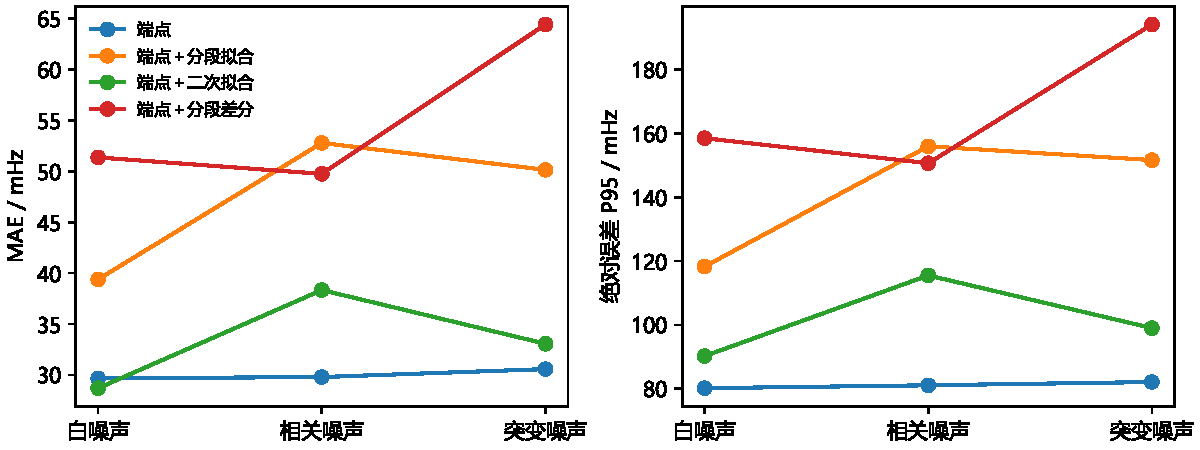
\includegraphics[width=.91\linewidth]{assets/noise-comparison.pdf}
\captionof{figure}{固定截止原噪声对照的绝对误差统计。各噪声结构采用相同物理事件。}
\end{center}

\section{等端点参数扫描}
固定$H=4$ s、$D=1$、$R=0.05$和调频上限0.1 p.u.。用$T_g=0.20$ s、三档参考缺额产生三个目标端点，在扰动缺额0.02至0.08 p.u.范围内，为四个较长的$T_g$匹配0.50 s端点。12组匹配均完成，端点误差小于$10^{-6}$ Hz，所记录样本均未触及调频上限。匹配同时改变缺额和调频时间常数。

\begin{center}
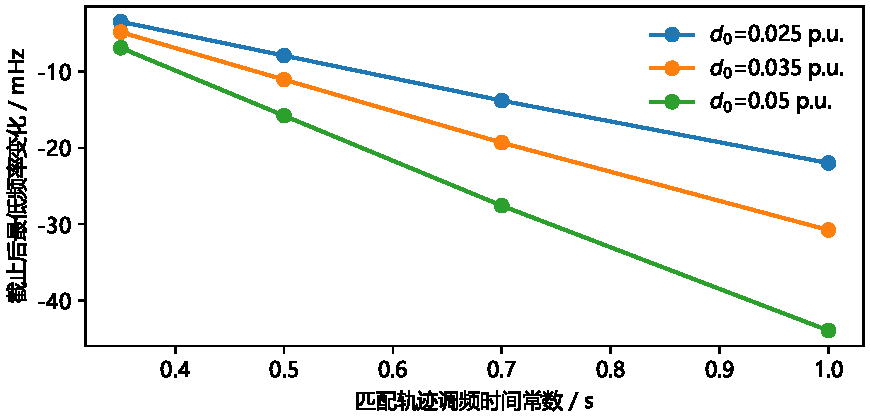
\includegraphics[width=.74\linewidth]{assets/endpoint-scan.pdf}
\captionof{figure}{等端点参数扫描的后缀极值差；每条曲线对应一个参考缺额。}
\end{center}

\section{单级与两级调频状态对照}
在500个既有配对场景中，按分段拟合绝对误差变化排序，取第10、50、95百分位秩的场景83、278、338。三对重算频率与保存轨迹的最大误差均低于0.05 mHz。点线表示调频目标，实线表示实际调频增功，竖虚线表示0.50 s截止线。三个案例的采样记录均未触及调频上限，两级结构的增功在响应初期较慢。两级结构对应的截止后最低值在三个案例中均下降，分段拟合的绝对误差变化分别为$-4.4$、5.6和31.2 mHz。

\begin{center}
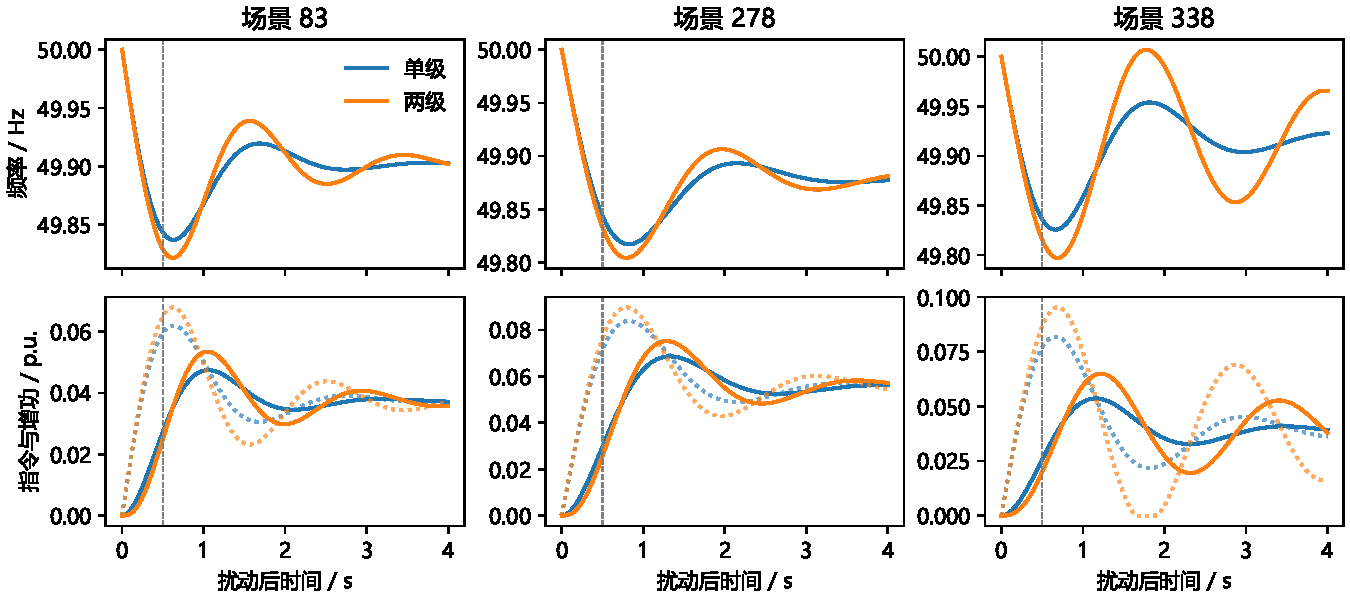
\includegraphics[width=\linewidth]{assets/structure-states.pdf}
\captionof{figure}{单级及两级调频结构的数值轨迹与调频响应对照。}
\end{center}

\section{个人电脑计算耗时}
在Intel Core i9-14900HX电脑上，对同一个测试场景预热后各测200次。特征提取采用MATLAB R2025a，推理采用Python 3.14.6与scikit-learn 1.9.0，推理含输入缩放。耗时单位为毫秒，本表对应单次软件调用。

\begin{center}
\begin{minipage}{\linewidth}\centering
\captionof{table}{本机计算耗时。耗时用于复现记录。}
\begin{tabular}{lrrrr}
\toprule
配置 & 特征中位 & 特征P95 & 推理中位 & 推理P95\\
\midrule
端点 & 0.0003 & 0.0013 & 0.170 & 0.296\\
端点加二次拟合 & 0.0047 & 0.0064 & 0.162 & 0.291\\
端点加分段差分 & 0.0007 & 0.0010 & 0.167 & 0.365\\
端点加分段拟合 & 0.0056 & 0.0061 & 0.158 & 0.266\\
\bottomrule
\end{tabular}
\end{minipage}
\end{center}

\section{等端点扫描与局部可辨识性}
扩展扫描以三档缺额为参考，每次改变惯量、阻尼或调频时间常数的一项，并在规定区间内调整缺额。36组中35组匹配成功。参考缺额为0.025 p.u.、惯量改为2.5 s的场景在原缺额范围内未匹配成功。图中横轴为匹配后两条可见频率轨迹的差值RMS，纵轴为两条轨迹的截止后最低频率绝对差。

对60个场景，以0.001和0.0005的两档对数参数步长计算中心差分。主汇总包含53个未限幅场景及其未限幅复本。每个场景以干净0.50 s窗频偏的均方根确定白噪声功率，跨窗口使用同一噪声标准差。通过特征算子行空间的正交基白化，保留特征共享样本引起的噪声相关性。过阈值方向的目标关联用截止后最低频率梯度在这些方向上的平方投影占比表示。两档步长的观测雅可比相对差中位数约为$1.0\times10^{-7}$，目标梯度约为$1.9\times10^{-7}$。梯度比较和缩放复核的逐场景结果随复现文件提供。

\begin{center}
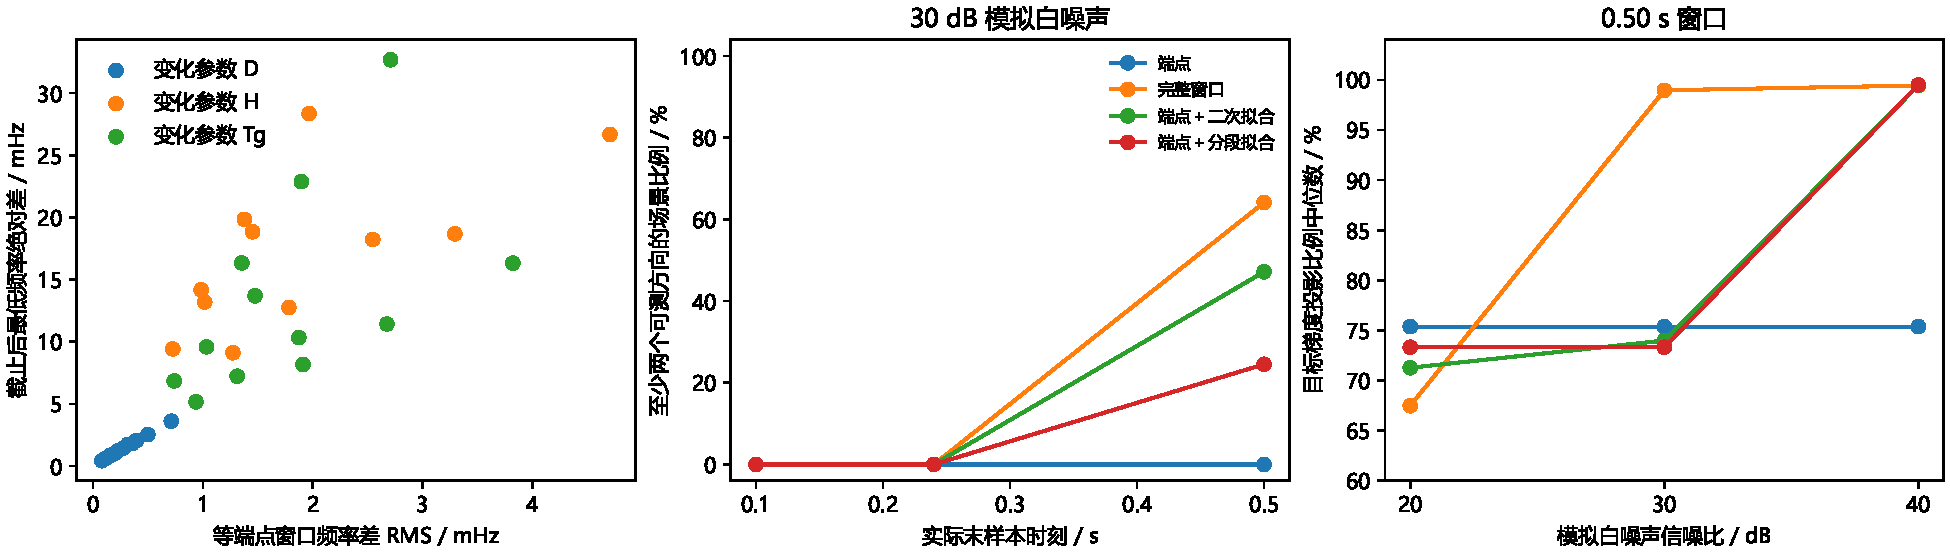
\includegraphics[width=\linewidth]{assets/matched-and-sensitivity.pdf}
\captionof{figure}{等端点匹配扫描及局部灵敏度指标。参数带与噪声条件依原协议。}
\par\small 等端点后目标差，以及不同窗长下的局部可测方向和目标投影。
\end{center}

\section{预测区间的分组与压力测试}
固定0.50 s二次拟合预测器。统一区间取尺度$\hat s=1$；分尺度区间以可见窗二阶差分均方根的开发集三分位点分组，各组用绝对残差中位数估计$\hat s(x)$。在独立的600例校准集上将$|y_i-\hat y_i|/\hat s(x_i)$升序排列，取第541项为$q$，区间为$[\hat y-q\hat s(x),\hat y+q\hat s(x)]$。两级调频与窗内突变试验共用原校准值。同分布测试中，分尺度区间的平均宽度减少35.7 mHz（配对95\%区间$[32.8,38.8]$），覆盖率下降2.0个百分点（$[1.1,3.0]$）。
分尺度方案的二阶差分均方根分界约为2.854与12.058 mHz，尺度为每组开发事件绝对残差中位数，设0.001 Hz下限。测试场景每个成员在同条件下共享点预测与标签。表中各条件的测试场景数分别为1200、403、379、418、1200、1200。噪声突变自0.26 s起使噪声标准差达到此前的3倍，全窗期望功率归一为名义20 dB。两级调频沿用混合量测条件。

\begin{center}
\small
\begin{minipage}{\linewidth}\centering
\captionof{table}{固定截止双侧区间的覆盖、宽度与偏向。}
\begin{tabular}{lrrrrrr}
\toprule
& \multicolumn{2}{c}{覆盖率/\%} & \multicolumn{2}{c}{平均宽度/mHz} & \multicolumn{2}{c}{上侧漏覆盖/\%}\\
条件 & 统一 & 分尺度 & 统一 & 分尺度 & 统一 & 分尺度\\
\midrule
同分布混合 & 92.5 & 90.5 & 152.7 & 117.0 & 5.83 & 7.50\\
干净量测 & 100.0 & 94.8 & 152.7 & 49.1 & 0.00 & 4.47\\
白噪声 & 90.2 & 91.8 & 152.7 & 165.1 & 8.44 & 7.39\\
相关噪声 & 87.3 & 85.2 & 152.7 & 138.7 & 9.09 & 10.53\\
噪声突变 & 88.1 & 90.8 & 152.7 & 164.1 & 10.00 & 8.08\\
两级调频 & 90.0 & 79.3 & 152.7 & 117.5 & 8.75 & 19.33\\
\bottomrule
\end{tabular}
\end{minipage}
\end{center}
\begin{center}
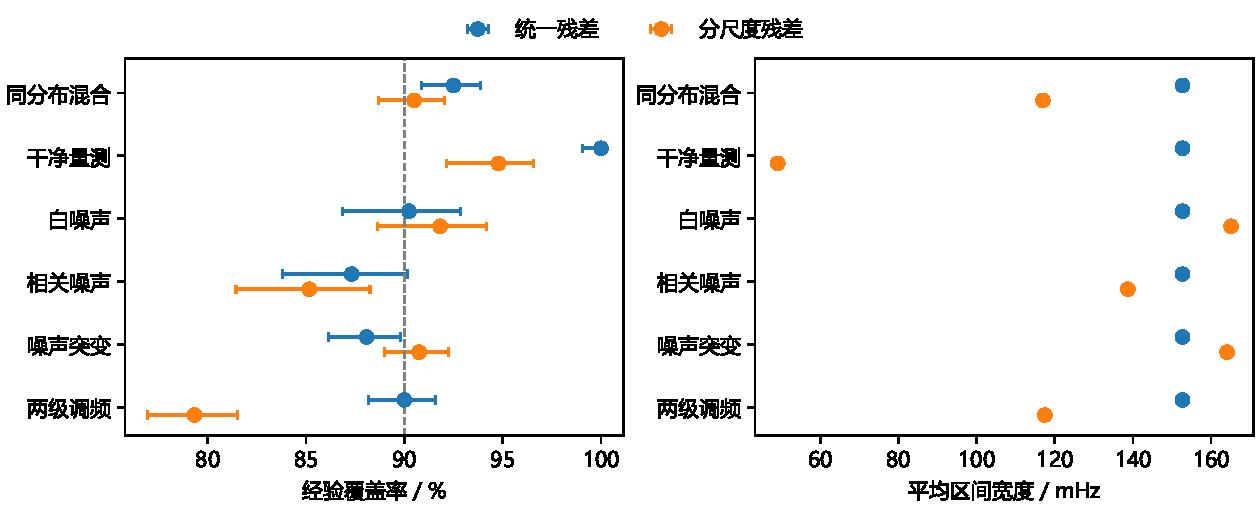
\includegraphics[width=.9\linewidth]{assets/coverage-width.pdf}
\captionof{figure}{固定截止双侧预测区间的覆盖与区间宽度。各组分母见相邻表。}
\par\small 各条件的经验覆盖率及其区间估计、平均预测区间宽度。
\end{center}

\clearpage
\section{独立近端点配对的完整结果}
\subsection{筛选流转与失败账本}
$R$带1为$[0.041,0.044]$，带2为$[0.056,0.059]$。表\ref{tab:s-flow}中，“主幅度”指可推理且真实绝对差不小于2.00 mHz的配对，“小差”指高于0.50 mHz且低于2.00 mHz的非并列对。真实并列和小差配对均参加方向评价。正式试验的几何匹配失败率为\PairMatchFailureRate{}\%。缺额无法括根、求根失败、仿真失败、超端点容差、与历史参数重合以及特征失败的计数均列在随附原因表和逐对账本中。

\begin{center}
\small
\captionof{table}{近端点配对的样本流转}
\label{tab:s-flow}
\begin{tabular}{llrrrrrrr}
\toprule
$R$带 & 因素 & 尝试 & 匹配 & 主幅度 & 真并列 & 小差 & 匹配失败 & 特征失败\\
\midrule
\resultrows{assets/pair-flow-rows.tex}
\bottomrule
\end{tabular}
\end{center}

\subsection{两种条件下的差值与方向评价}
表\ref{tab:s-metrics}的误差均按主幅度集合计算，方向分母纳入全部可推理配对。白噪声行按每对10个复本计算。“真并列”列在白噪声行也按次数报告，对应同一个真实并列事件。模型栏沿用主稿定义。白噪声均指30 dB模拟高斯白噪声。

\begin{center}
\small
\captionof{table}{总体误差与方向指标}
\label{tab:s-metrics}
\setlength{\tabcolsep}{4pt}
\begin{tabular}{llrrrrrr}
\toprule
条件 & 输入 & MAE/mHz & RMSE/mHz & P95/mHz & 判对/总数 & 预测并列 & 真并列\\
\midrule
\resultrows{assets/pair-summary-rows.tex}
\bottomrule
\end{tabular}
\end{center}

\clearpage
\subsection{配对效应与下垂系数分带统计}
表\ref{tab:s-effects}列出同一候选配对上的差值MAE变化，正数表示误差增加。各区间用主稿的分层参考事件重采样口径。表\ref{tab:s-bands}用于描述两参数带的结果。

\begin{center}
\small
\captionof{table}{相对两个基线的差值MAE变化及95\%区间（mHz）}
\label{tab:s-effects}
\begin{tabular}{llll}
\toprule
条件 & 输入 & 比较基线 & 变化及区间\\
\midrule
\resultrows{assets/pair-effect-rows.tex}
\bottomrule
\end{tabular}
\end{center}

\begin{center}
\small
\captionof{table}{下垂系数分带结果}
\label{tab:s-bands}
\setlength{\tabcolsep}{3pt}
\begin{tabular}{lllrrrrrrr}
\toprule
$R$带 & 条件 & 输入 & 主对数 & MAE & RMSE & P95 & 相对端点变化 & 判对/总数 & 预测并列\\
\midrule
\resultrows{assets/pair-band-rows.tex}
\bottomrule
\end{tabular}
\par\smallskip
\footnotesize 误差及误差变化单位为mHz。每带的真并列物理对数见表\ref{tab:s-flow}。
\end{center}

\clearpage
\subsection{原网格随机划分与复算记录}
原网格的十次随机划分复用同一仿真场景集。表\ref{tab:s-repeat}中的标准差反映划分敏感性。

\begin{center}
\small
\captionof{table}{十次随机划分的梯度提升树结果}
\label{tab:s-repeat}
\begin{tabular}{lrr}
\toprule
特征 & 均方根误差/Hz & $R^2$\\
\midrule
\resultrows{revision-assets/repeat.tex}
\bottomrule
\end{tabular}
\end{center}

近端点正式试验的参考参数表和配对账本记录参考与候选标识、配对参数、截点及目标频差、匹配状态和排除原因。逐对预测表保留成员预测、真实差和预测差、方向及并列字段。复算按参考事件和候选标识对齐成员，严格从观测截止后采样重新核对标签，重新判定三类方向与幅度纳入状态。重采样在两个下垂系数带内分别抽取参考事件，同一参考的候选和噪声复本共同进出。随附核验日志记载逐指标校验与5\,000个重采样结果的复核。历史基准检查表记录固定0.50 s窗口特征及逐场景预测相对原档案的误差。

\section{复现入口}
数字对照表列出正式CSV的筛选键、字段、计算式和单位。配对证据文件与补充材料一并提供。原有实验的复现入口如下。
随稿说明给出原有仿真与模型训练的复现入口。短窗矩阵、边界事件、扩展噪声、局部可辨识性及预测区间均保留原始实验记录。
\clearpage
\section{ECGR与门控的独立确认样本流转与稳健性口径}
ECGR确认由\Erefs{}个参考场景形成\Epairs{}对，主幅值分析\Eeligible{}对。门控确认由\Prefs{}个参考场景形成\Pcount{}对，主幅值分析\Peligible{}对；独立单场景\Srefs{}个。两次确认使用不同种子和参数。所有含噪复本随对应物理事件进入聚类重采样。方向计数以全部可评分配对为分母，误差表的幅值集合按预设目标差筛选。各条件、阶段的原始样本流转、匹配状态及阈值保存在配套证据表。正常匹配但真实差不足的配对单列；方向评价保留真实并列。配对真值差与预测差均按候选减参考，带符号的差值误差取预测差减真值差。

两个确认试验都将未加噪端点差容差定为0.10 mHz。每个参考场景依次调整 \(H\)、\(D\) 或 \(T_g\)，再对功率缺额求根使候选端点与参考端点吻合；配对两成员的全局最低点均在截止以后。两带调差系数范围为 \([0.041,0.044]\) 与 \([0.056,0.059]\)。配对的构造变量只用于离线生成与分组。ECGR的方向集合包括6个真实并列和60个小差非并列；门控的方向集合包括2个真实并列和66个小差非并列。上述配对均保留在方向分母中。

\section{ECGR的完整配对指标}
\small
\begin{longtable}{llrrrr}
\caption{固定截止ECGR确认中的配对差值指标。}\\
\toprule
条件 & 模型 & MAE & RMSE & P95 & 方向判对/总数 \\
\midrule
\endfirsthead
\toprule
条件 & 模型 & MAE & RMSE & P95 & 方向判对/总数 \\
\midrule
\endhead
干净 & ECGR & 4.44 & 5.89 & 11.20 & 234/288 \\
干净 & 端点 & 11.22 & 12.63 & 22.04 & 6/288 \\
干净 & 分段拟合 & 7.20 & 9.37 & 19.52 & 228/288 \\
干净 & 初始斜率 & 11.29 & 14.41 & 23.78 & 109/288 \\
干净 & 二次拟合 & 5.67 & 7.79 & 14.89 & 246/288 \\
白噪30 dB & ECGR & 13.96 & 19.11 & 39.57 & 1967/2880 \\
白噪30 dB & 端点 & 14.00 & 17.55 & 34.33 & 940/2880 \\
白噪30 dB & 分段拟合 & 17.99 & 24.35 & 49.69 & 1831/2880 \\
白噪30 dB & 初始斜率 & 23.62 & 32.67 & 69.03 & 1482/2880 \\
白噪30 dB & 二次拟合 & 13.71 & 18.66 & 39.09 & 1944/2880 \\
\bottomrule
\end{longtable}
\normalsize 各表误差及损失单位为mHz。

数据表还提供独立确认的单场景误差、ECGR相对四类固定配置的聚类区间、冻结阈值及未通过项。三次系数训练尺度为 \(\ECubicMoment\times10^{-5}\) Hz$^2$，以未收缩系数平方的训练集均值计算。配套单元检查涵盖零残差、仿射窗、白噪声和相关噪声的协方差传播。
\clearpage
\section{门控逐条件完整指标}
\small
\begin{longtable}{lllrrrr}
\caption{固定截止质量门控的逐条件确认指标。}\\
\toprule
任务 & 条件 & 模型 & MAE & RMSE & P95 & 方向判对/总数 \\
\midrule
\endfirsthead
\toprule
任务 & 条件 & 模型 & MAE & RMSE & P95 & 方向判对/总数 \\
\midrule
\endhead
单场景 & AR(1) 30 dB & 端点 & 23.25 & 30.43 & 63.85 & — \\
单场景 & AR(1) 30 dB & 初始斜率 & 19.46 & 26.74 & 53.74 & — \\
单场景 & AR(1) 30 dB & 二次拟合 & 18.64 & 27.06 & 60.82 & — \\
单场景 & AR(1) 30 dB & 分段拟合 & 20.16 & 28.44 & 60.29 & — \\
单场景 & AR(1) 30 dB & ECGR & 18.87 & 27.32 & 62.54 & — \\
单场景 & AR(1) 30 dB & 门控 & 23.20 & 30.35 & 63.83 & — \\
单场景 & 干净 & 端点 & 23.68 & 31.36 & 67.96 & — \\
单场景 & 干净 & 初始斜率 & 15.06 & 19.05 & 39.26 & — \\
单场景 & 干净 & 二次拟合 & 9.63 & 13.00 & 27.83 & — \\
单场景 & 干净 & 分段拟合 & 10.25 & 13.02 & 28.16 & — \\
单场景 & 干净 & ECGR & 8.24 & 10.85 & 21.51 & — \\
单场景 & 干净 & 门控 & 8.24 & 10.85 & 21.51 & — \\
单场景 & 突变 & 端点 & 24.86 & 32.20 & 65.95 & — \\
单场景 & 突变 & 初始斜率 & 36.89 & 53.13 & 115.59 & — \\
单场景 & 突变 & 二次拟合 & 38.49 & 54.45 & 122.08 & — \\
单场景 & 突变 & 分段拟合 & 51.41 & 71.47 & 162.71 & — \\
单场景 & 突变 & ECGR & 39.17 & 56.53 & 125.26 & — \\
单场景 & 突变 & 门控 & 24.95 & 32.32 & 66.18 & — \\
单场景 & 白噪20 dB & 端点 & 24.97 & 32.61 & 66.58 & — \\
单场景 & 白噪20 dB & 初始斜率 & 40.83 & 59.55 & 126.97 & — \\
单场景 & 白噪20 dB & 二次拟合 & 29.97 & 42.40 & 93.30 & — \\
单场景 & 白噪20 dB & 分段拟合 & 40.56 & 57.32 & 121.83 & — \\
单场景 & 白噪20 dB & ECGR & 31.88 & 46.01 & 98.83 & — \\
单场景 & 白噪20 dB & 门控 & 24.97 & 32.61 & 66.58 & — \\
单场景 & 白噪30 dB & 端点 & 23.48 & 30.70 & 63.26 & — \\
单场景 & 白噪30 dB & 初始斜率 & 21.36 & 29.66 & 59.66 & — \\
单场景 & 白噪30 dB & 二次拟合 & 14.52 & 20.38 & 44.63 & — \\
单场景 & 白噪30 dB & 分段拟合 & 17.07 & 23.83 & 51.68 & — \\
单场景 & 白噪30 dB & ECGR & 15.40 & 21.75 & 46.19 & — \\
单场景 & 白噪30 dB & 门控 & 23.48 & 30.70 & 63.26 & — \\
单场景 & 白噪40 dB & 端点 & 23.32 & 30.46 & 64.59 & — \\
单场景 & 白噪40 dB & 初始斜率 & 16.26 & 20.87 & 39.51 & — \\
单场景 & 白噪40 dB & 二次拟合 & 10.57 & 14.13 & 30.28 & — \\
单场景 & 白噪40 dB & 分段拟合 & 11.15 & 14.39 & 28.99 & — \\
单场景 & 白噪40 dB & ECGR & 11.03 & 14.40 & 27.52 & — \\
单场景 & 白噪40 dB & 门控 & 10.66 & 14.24 & 30.72 & — \\
配对 & AR(1) 30 dB & 端点 & 14.86 & 18.91 & 37.73 & 897/2880 \\
配对 & AR(1) 30 dB & 初始斜率 & 22.89 & 31.80 & 70.49 & 1503/2880 \\
配对 & AR(1) 30 dB & 二次拟合 & 21.36 & 29.45 & 61.37 & 1795/2880 \\
配对 & AR(1) 30 dB & 分段拟合 & 23.41 & 31.50 & 64.62 & 1754/2880 \\
配对 & AR(1) 30 dB & ECGR & 20.68 & 28.37 & 58.64 & 1805/2880 \\
配对 & AR(1) 30 dB & 门控 & 14.89 & 18.96 & 38.05 & 906/2880 \\
配对 & 干净 & 端点 & 12.24 & 13.70 & 22.81 & 2/288 \\
配对 & 干净 & 初始斜率 & 11.94 & 14.09 & 23.50 & 108/288 \\
配对 & 干净 & 二次拟合 & 6.08 & 8.25 & 16.33 & 246/288 \\
配对 & 干净 & 分段拟合 & 7.55 & 9.52 & 19.30 & 211/288 \\
配对 & 干净 & ECGR & 4.72 & 6.36 & 13.11 & 240/288 \\
配对 & 干净 & 门控 & 4.72 & 6.36 & 13.11 & 240/288 \\
配对 & 突变 & 端点 & 19.40 & 25.01 & 49.78 & 1230/2880 \\
配对 & 突变 & 初始斜率 & 45.05 & 61.72 & 132.51 & 1513/2880 \\
配对 & 突变 & 二次拟合 & 49.16 & 66.14 & 141.46 & 1568/2880 \\
配对 & 突变 & 分段拟合 & 67.14 & 90.46 & 195.35 & 1553/2880 \\
配对 & 突变 & ECGR & 49.55 & 67.02 & 145.63 & 1560/2880 \\
配对 & 突变 & 门控 & 19.40 & 25.01 & 49.78 & 1230/2880 \\
配对 & 白噪20 dB & 端点 & 19.00 & 25.09 & 47.80 & 1220/2880 \\
配对 & 白噪20 dB & 初始斜率 & 49.25 & 67.61 & 147.15 & 1416/2880 \\
配对 & 白噪20 dB & 二次拟合 & 40.03 & 54.22 & 110.66 & 1629/2880 \\
配对 & 白噪20 dB & 分段拟合 & 51.43 & 68.57 & 148.12 & 1589/2880 \\
配对 & 白噪20 dB & ECGR & 41.92 & 57.29 & 120.39 & 1611/2880 \\
配对 & 白噪20 dB & 门控 & 19.00 & 25.09 & 47.80 & 1220/2880 \\
配对 & 白噪30 dB & 端点 & 14.75 & 18.56 & 35.51 & 925/2880 \\
配对 & 白噪30 dB & 初始斜率 & 25.27 & 36.08 & 80.47 & 1477/2880 \\
配对 & 白噪30 dB & 二次拟合 & 15.40 & 20.93 & 44.36 & 1977/2880 \\
配对 & 白噪30 dB & 分段拟合 & 18.23 & 24.48 & 49.43 & 1821/2880 \\
配对 & 白噪30 dB & ECGR & 15.83 & 21.57 & 45.07 & 1926/2880 \\
配对 & 白噪30 dB & 门控 & 14.75 & 18.56 & 35.51 & 925/2880 \\
配对 & 白噪40 dB & 端点 & 13.20 & 16.00 & 27.03 & 566/2880 \\
配对 & 白噪40 dB & 初始斜率 & 14.69 & 19.37 & 37.98 & 1316/2880 \\
配对 & 白噪40 dB & 二次拟合 & 7.73 & 10.33 & 21.02 & 2298/2880 \\
配对 & 白噪40 dB & 分段拟合 & 9.08 & 11.47 & 22.27 & 2091/2880 \\
配对 & 白噪40 dB & ECGR & 7.50 & 9.95 & 20.54 & 2287/2880 \\
配对 & 白噪40 dB & 门控 & 7.85 & 10.56 & 21.23 & 2289/2880 \\
\bottomrule
\end{longtable}
\normalsize 各表误差及损失单位为mHz。

\clearpage
\section{事后诊断和突变案例}
\small
\begin{longtable}{llrrr}
\caption{固定截止门控的误选与误选损失诊断。}\\
\toprule
任务 & 条件 & 误选率/\% & 平均损失 & P95损失 \\
\midrule
\endfirsthead
\toprule
任务 & 条件 & 误选率/\% & 平均损失 & P95损失 \\
\midrule
\endhead
单场景 & AR(1) 30 dB & 68.20 & 12.50 & 47.88 \\
单场景 & 干净 & 53.91 & 2.06 & 11.03 \\
单场景 & 突变 & 42.97 & 8.20 & 41.22 \\
单场景 & 白噪20 dB & 52.42 & 9.84 & 42.63 \\
单场景 & 白噪30 dB & 74.30 & 14.18 & 50.02 \\
单场景 & 白噪40 dB & 59.38 & 3.42 & 14.21 \\
配对 & AR(1) 30 dB & 80.86 & 8.95 & 26.75 \\
配对 & 干净 & 80.00 & 2.76 & 9.18 \\
配对 & 突变 & 62.59 & 8.49 & 33.00 \\
配对 & 白噪20 dB & 67.77 & 9.20 & 32.86 \\
配对 & 白噪30 dB & 84.27 & 9.63 & 25.77 \\
配对 & 白噪40 dB & 87.00 & 5.13 & 16.09 \\
\bottomrule
\end{longtable}
\normalsize 各表误差及损失单位为mHz。

\begin{center}
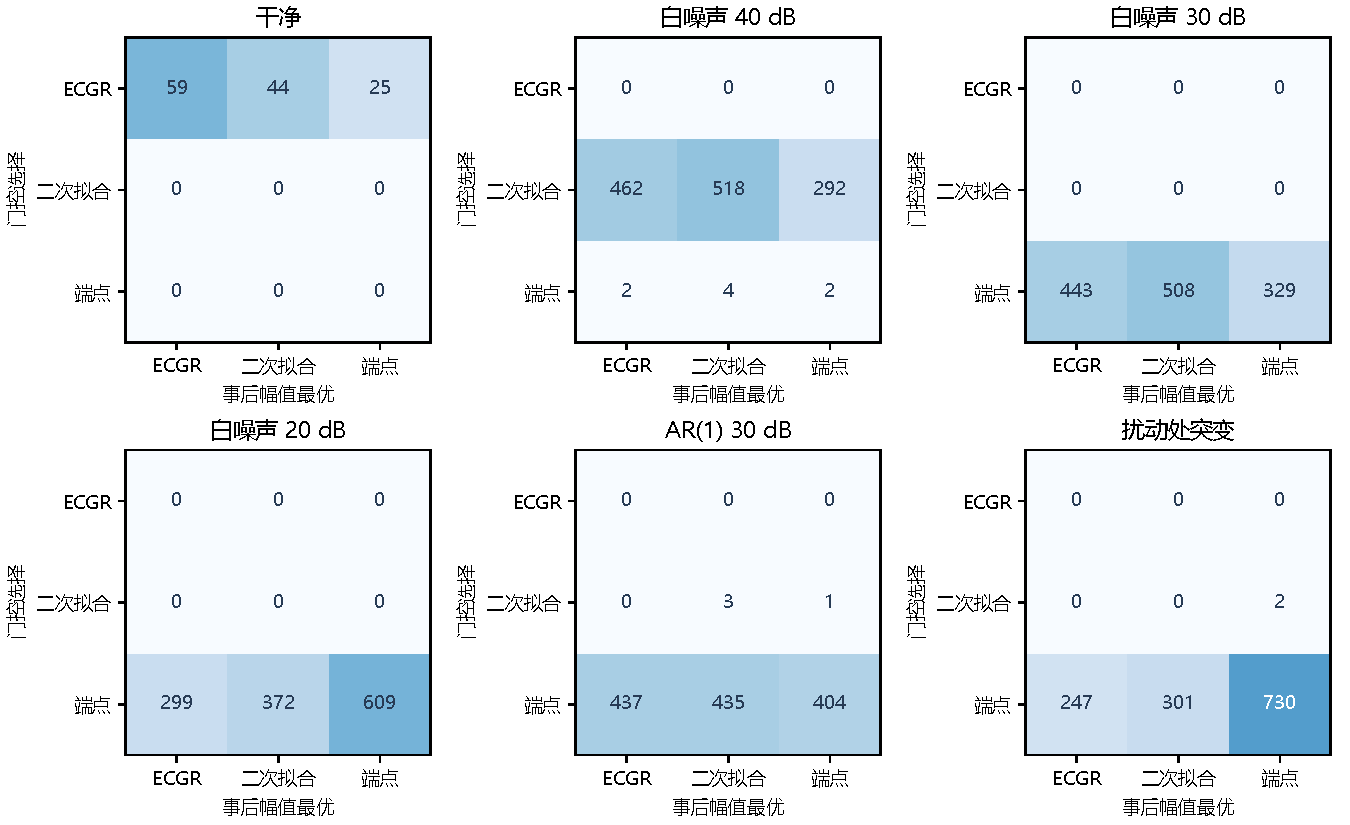
\includegraphics[width=.75\linewidth]{quality-assets/figures/quality-misselection-matrix.pdf}
\captionof{figure}{单场景实际选择与事后误差最小表示的混淆矩阵。}
\end{center}
\clearpage
\begin{center}
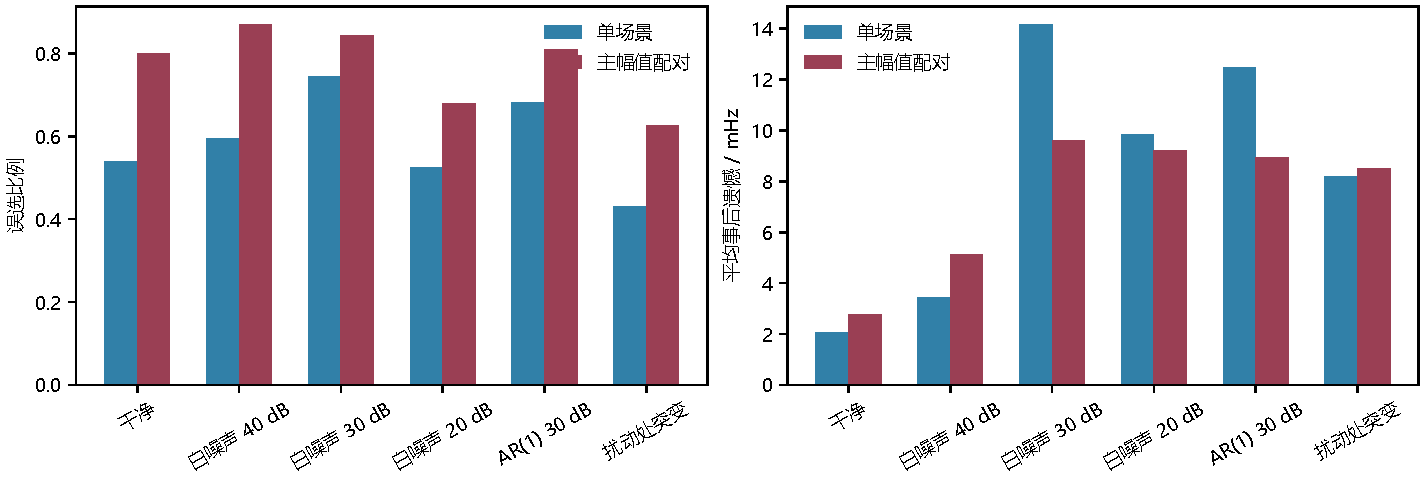
\includegraphics[width=.92\linewidth]{quality-assets/figures/quality-misselection-loss.pdf}
\captionof{figure}{单场景及主幅值配对的误选率与超过事后最优的损失。}
\end{center}
\begin{center}
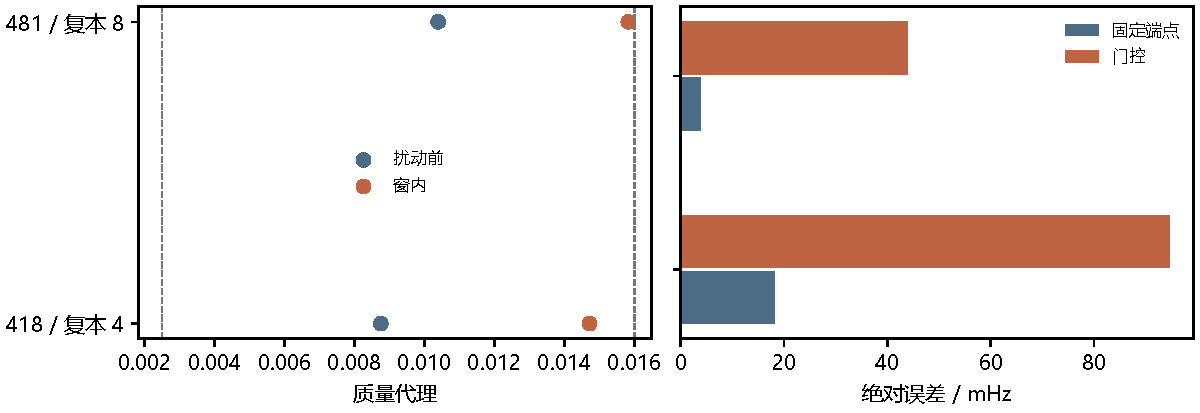
\includegraphics[width=.92\linewidth]{quality-assets/figures/jump-failures.pdf}
\captionof{figure}{突变中两例选择二次拟合的单场景。左图同时显示可观测代理和冻结阈值；右图按预测值及真值计算绝对误差。案例从正式预测筛选，无新增仿真。}
\end{center}
\section{复现与统计核对}
原估计器和门控的冻结记录均包含源文件指纹。只读审计按事件键复算单场景和配对指标。近端点目标差与成员预测差保持同一方向，先以Hz相减再换算mHz。聚类抽样以独立单场景或配对参考事件为单位，并按下垂系数带分层。各固定基线共享观测与目标。事后诊断允许访问真值，只用于计算误选和损失。两条编号链及逐场景输出的入口见随稿复现说明。

\clearpage
\section{滚动策略对照与时序扰动的完整结果}
四时刻联合下界用独立校准事件的最大标准化误差取得统一分位数，开发集确定各时刻尺度。干净测试的四时刻联合覆盖率为90.25\%。该项覆盖与滚动事件级命中率分别评价，也与单侧固定截止负面试验采用不同标签和校准集。

两种时序误差只改变输入的采样位置，事件真值依真实扰动时间轴定义。

\begin{table}[!htbp]\centering\small
\caption{干净聚合滚动试验的完整策略对照，5\%校准目标}\label{tab:full-roll}
\begin{tabular}{lrrrr}\toprule 策略 & 及时命中 & 虚警 & 实际虚警率/\% & 中位提前量/ms\\ \midrule
持续性滚动 & 219/291 & 99/1309 & 7.6 & 160 \\
端点滚动 & 142/291 & 62/1309 & 4.7 & 140 \\
二次拟合滚动 & 272/291 & 84/1309 & 6.4 & 390 \\
分段斜率滚动 & 272/291 & 92/1309 & 7.0 & 340 \\
二次拟合固定时刻 & 189/291 & 74/1309 & 5.7 & 240 \\
二次拟合联合下界滚动 & 267/291 & 73/1309 & 5.6 & 380 \\
\bottomrule\end{tabular}\end{table}
\begin{table}[!htbp]\centering\small
\caption{冻结阈值下二次拟合滚动策略的时序与噪声压力结果}\label{tab:full-stress}
\begin{tabular}{lrrrr}\toprule 条件 & 及时命中 & 虚警 & 实际虚警率/\% & 中位提前量/ms\\ \midrule
20 dB & 270/291 & 573/1309 & 43.8 & 340 \\
30 dB & 282/291 & 403/1309 & 30.8 & 340 \\
40 dB & 283/291 & 245/1309 & 18.7 & 360 \\
起点偏早20 ms & 290/291 & 568/1309 & 43.4 & 440 \\
起点偏晚20 ms & 290/291 & 162/1309 & 12.4 & 400 \\
起点偏早40 ms & 289/291 & 522/1309 & 39.9 & 460 \\
起点偏晚40 ms & 291/291 & 239/1309 & 18.3 & 380 \\
20 dB、偏晚40 ms、时延20 ms & 277/291 & 686/1309 & 52.4 & 300 \\
\bottomrule\end{tabular}\end{table}
\begin{center}
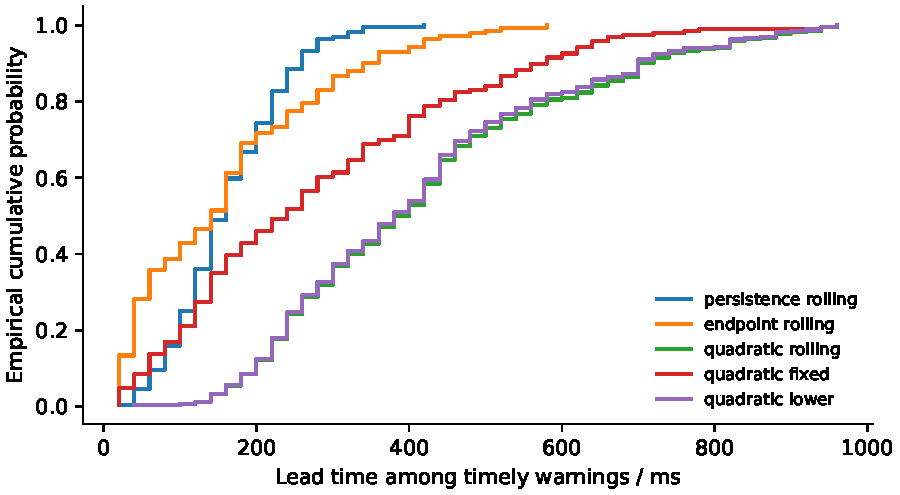
\includegraphics[width=.46\linewidth]{rolling-figures/lead.pdf}\hfill
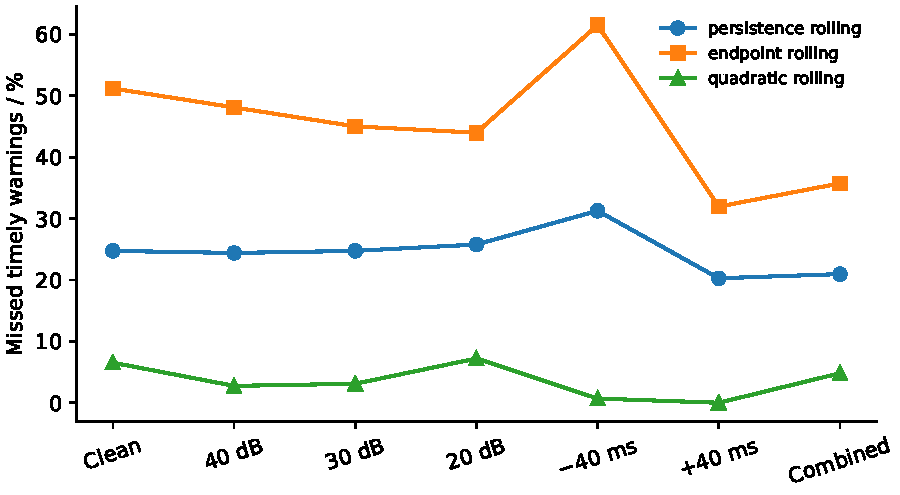
\includegraphics[width=.46\linewidth]{rolling-figures/stress.pdf}
\captionof{figure}{滚动告警提前量分布（左）与扰动敏感性（右）。}
\end{center}
\clearpage
\section{多机滚动预警的前期压力试验}
以下试验为在正式高负荷及位置留出确认前开展的数值压力诊断，与主文后续确认批次分别解释。采用 ANDES 2.0 对公开 IEEE 动态算例进行负荷阶跃试验。扰动幅度按初始总负荷的1.5\%至12\%设置。以惯量中心频率定义越限，分别使用惯量中心频率、一个母线量测及三个母线量测的均值作为输入。模型及阈值从聚合试验直接迁移。IEEE 14节点完成90/90组，IEEE 39节点完成80/90组。其余10组时域积分未收敛，保留在场景表中，直接迁移对照统计仅使用完成的仿真。大扰动的结果可能受可收敛场景选择影响。14节点只有2个越限事件，39节点可评分场景没有越限事件，因而本组数据无法确认跨系统漏报表现。
\begin{center}
\small\setlength{\tabcolsep}{5pt}
\captionof{table}{早期多机算例的直接迁移对照，按可评分场景计数。}
\begin{tabular}{lrrrrrr}
\toprule
配置 & 场景数 & 越限 & 按时命中 & 虚警率/\% & 未按时告警/\% & 中位提前量/ms\\
\midrule
ieee14\_coi & 90 & 2 & 1 & 0.0 & 50.0 & 1220 \\
ieee14\_single & 90 & 2 & 0 & 0.0 & 100.0 & -- \\
ieee14\_multi & 90 & 2 & 0 & 0.0 & 100.0 & -- \\
ieee39\_coi & 80 & 0 & 0 & 0.0 & -- & -- \\
ieee39\_single & 80 & 0 & 0 & 0.0 & -- & -- \\
ieee39\_multi & 80 & 0 & 0 & 0.0 & -- & -- \\
\bottomrule
\end{tabular}
\end{center}

\subsection{分布式负荷阶跃与阈值迁移}
为增加可评分的越限事件，另在多个负荷母线上按原有负荷比例施加同步阶跃，按0.94、1.00和1.06倍基准负荷组织场景，阶跃总量为扰动前系统负荷的8.5\%至17.5\%。该试验为有意加重的压力测试。14和39节点分别完成90/90和56/90组。模型保持冻结。以1.00倍负荷的未越限事件校准本地阈值，在0.94和1.06倍负荷的独立场景报告结果。分布式阶跃对照同时列出沿用聚合阈值与应用本地校准阈值的表现。

\begin{center}
\small\setlength{\tabcolsep}{5pt}
\captionof{table}{IEEE 14及39节点分布式阶跃的预警与本地校准。}
\begin{tabular}{lrrrrrr}
\toprule
配置 & 场景数 & 越限 & 按时命中 & 虚警率/\% & 未按时告警/\% & 中位提前量/ms\\
\midrule
14节点惯量中心（迁移） & 60 & 32 & 30 & 0.0 & 6.2 & 840 \\
14节点惯量中心（本地） & 60 & 32 & 30 & 0.0 & 6.2 & 840 \\
14节点多点均值（迁移） & 60 & 32 & 0 & 0.0 & 100.0 & -- \\
14节点多点均值（本地） & 60 & 32 & 27 & 3.6 & 15.6 & 520 \\
39节点惯量中心（迁移） & 37 & 6 & 0 & 0.0 & 100.0 & -- \\
39节点惯量中心（本地） & 37 & 6 & 6 & 3.2 & 0.0 & 1740 \\
39节点多点均值（迁移） & 37 & 6 & 0 & 0.0 & 100.0 & -- \\
39节点多点均值（本地） & 37 & 6 & 4 & 3.2 & 33.3 & 1440 \\
\bottomrule
\end{tabular}
\end{center}


以多点均值为输入时，直接移植聚合阈值在两个算例中均无及时命中。使用本地阈值后，二次拟合在14节点命中27/32并产生1次虚警，在39节点命中4/6并产生1次虚警。同样校准的持续性基线分别命中32/32和6/6，各产生2次虚警。现有样本支持本地校准对直接迁移的改善，尚不足以判定二次拟合在相同虚警水平下优于持续性。加入等效20 dB噪声后，二次拟合本地阈值的虚警分别增至7次和10次。

两个算例的本地校准仅分别包含14和15个未越限事件，无法精细匹配5\%虚警目标。测试结果应结合逐场景计数和汇总文件中的区间解释。未收敛场景不参与性能计算，39节点可评分结果可能受收敛性筛选影响。

\subsection{IEEE 39节点追加场景与噪声校准}
依据前轮结果，在两个较易产生可评分越限事件的多母线负荷分布上补充试验。采用6个初始负荷水平，每组分别在负荷阶跃比0.093至0.121及0.128至0.147的区间内随机抽取4个幅值。计划96组，完成92组。0.945、0.985和1.035倍负荷仅用于阈值选择，0.965、1.015和1.055倍负荷用于评估。持续性和二次拟合的模型结构保持固定。

追加场景噪声校准对照以多点均值量测、10\%目标虚警率为主要对照。5\%与20\%目标的结果同时保存在附件。噪声匹配阈值由同噪声水平的独立校准场景得到，且量测噪声水平在本试验中已知。IEEE 39节点的非收敛场景完整记录，该组评价针对特意增强越限覆盖的压力测试。

\begin{center}
\small\setlength{\tabcolsep}{5pt}
\captionof{table}{IEEE 39追加场景的预警与匹配噪声校准。}
\begin{tabular}{p{3.95cm}rrrrrr}
\toprule
配置 & 场景数 & 越限 & 按时命中 & 虚警率/\% & 未按时告警/\% & 中位提前量/ms\\
\midrule
持续性／干净量测／干净校准 & 45 & 17 & 17 & 10.7 & 0.0 & 1460 \\
二次拟合／干净量测／干净校准 & 45 & 17 & 14 & 7.1 & 17.6 & 1470 \\
持续性／等效20 dB／干净校准 & 45 & 17 & 15 & 17.9 & 11.8 & 1480 \\
持续性／等效20 dB／同噪声校准 & 45 & 17 & 7 & 0.0 & 58.8 & 1380 \\
二次拟合／等效20 dB／干净校准 & 45 & 17 & 11 & 35.7 & 35.3 & 1660 \\
二次拟合／等效20 dB／同噪声校准 & 45 & 17 & 10 & 17.9 & 41.2 & 1670 \\
\bottomrule
\end{tabular}
\end{center}


新增场景共92组可评分，其中35组越限。封存测试含45组，其中17组越限。干净量测下，持续性与二次拟合分别及时命中17和14组，虚警分别为3和2次。等效20 dB噪声下，匹配噪声校准使二次拟合虚警从10次降至5次，及时命中从11组降至10组。持续性的虚警从5次降至0次，及时命中由15组降至7组。相同目标虚警率未产生相同的实际虚警率，现有样本体现的是漏报与虚警之间的权衡。定向算例结果仅适用于本组扰动分布。

\subsection{固定物理场景上的噪声实现敏感性}
在一组固定的IEEE 39节点校准与测试场景上，更换40个随机噪声实现，逐实现重新选择告警阈值。二次拟合使用目标系统校准数据训练，其阈值基于校准集的五折折外预测。各实现包含21个物理越限事件及每个事件的6种量测条件，每实现共有126个越限场景与量测条件组合。四条件混合试验仍采用前文口径。

\noindent\begin{minipage}{\linewidth}
\begin{center}
\captionof{table}{前期IEEE 39固定场景的40个噪声实现，10\%目标虚警下的平均及时命中。}
\begin{tabular}{lrrr}
\toprule
比较 & 持续性 & 二次拟合 & 残差 \\
\midrule
平均命中数 & 107.03 & 102.03 & 79.08 \\
\bottomrule
\end{tabular}
\end{center}
\end{minipage}

二次拟合较持续性平均少5.00个及时命中，按实现配对的95\%区间为$[-6.75,-3.25]$。二次拟合在6/40个实现中反超，表明平均方向未在全部实现保持。按实际虚警率对齐后的插值比较得到平均差$-14.37$个命中，95\%区间为$[-17.61,-11.14]$；其中4个实现需使用曲线端点处理。这项插值用于诊断工作点差异。按21个物理越限事件进行簇重采样估计，持续性的设计效应为1.48（95\%区间$[1.26,1.61]$），区间跨越离散度判据所需的1.36。结果限于固定的物理场景、模型及噪声族。

\begin{center}
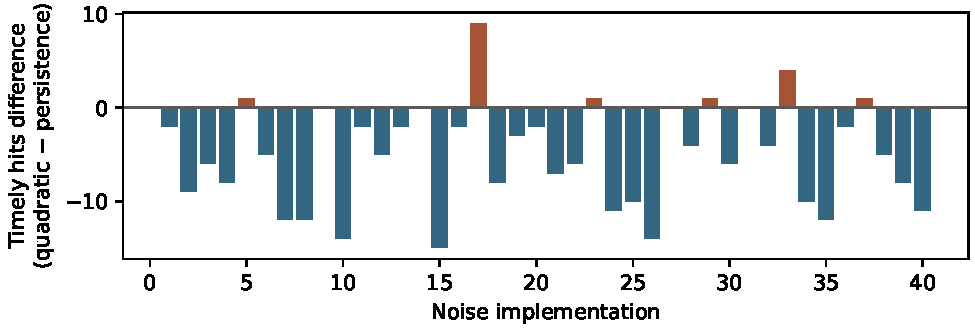
\includegraphics[width=.82\linewidth]{rolling-figures/r2-paired-noise.pdf}
\captionof{figure}{前期多机固定场景中的40个噪声实现，二次拟合减持续性的及时命中计数。每个实现有126个越限组合。}
\end{center}

\subsection{负荷外推与未见扰动位置}
另外生成144组新的IEEE 39节点场景，完成139组。阈值仅由目标系统校准块确定。主测试块的四个负荷水平全部位于校准范围之外，且扰动位置沿用校准设计。次测试块在校准负荷范围内使用新负荷水平和未见母线组合。二次拟合与残差模型均在原聚合开发网格上训练，三类策略共享R3的量测、分级阈值规则和四个决策时刻。残差模型从测得的当前频率减去预测的额外跌幅。与上一小节的二次拟合训练口径存在差异，各轮结果独立解释。


\begin{center}
\footnotesize\setlength{\tabcolsep}{3pt}
\captionof{table}{早期未见物理场景的事件级滚动预警，10\%校准目标。}
\begin{tabular}{llrrrrrrr}
\toprule
测试块 & 策略 & 物理场景 & 物理越限 & 命中 & 虚警 & 命中率/\% & 虚警率/\% & 中位提前量/ms\\
\midrule
负荷外推 & 持续性 & 59 & 7 & 21 & 17 & 75.0 & 8.2 & 1300 \\
负荷外推 & 二次拟合 & 59 & 7 & 10 & 18 & 35.7 & 8.7 & 1390 \\
负荷外推 & 残差 & 59 & 7 & 20 & 26 & 71.4 & 12.5 & 1340 \\
扰动位置留出 & 持续性 & 16 & 3 & 10 & 8 & 83.3 & 15.4 & 1500 \\
扰动位置留出 & 二次拟合 & 16 & 3 & 3 & 3 & 25.0 & 5.8 & 1640 \\
扰动位置留出 & 残差 & 16 & 3 & 4 & 2 & 33.3 & 3.8 & 1640 \\
\bottomrule
\end{tabular}
\end{center}

早期留出对照的命中及虚警次数以场景与量测条件组合为单位。实际虚警率不同的工作点需结合另两档预设目标及按物理事件重采样的区间比较。试验结果仅代表本设计范围，收敛失败场景保留在设计记录中。

在负荷外推主测试中，持续性和二次拟合的实际虚警率分别为8.2\%和8.7\%。二次拟合相对持续性的及时命中率配对差为-39.3个百分点（95\%事件簇重采样区间$[-56.2,-25.0]$）。残差的实际虚警率为12.5\%，与持续性的工作点存在差异。次测试块只有少量物理越限事件，且新负荷水平与新扰动位置同时变化，结果用于诊断联合迁移。

\section{场景筛选与求解诊断}
以下诊断沿用主文高负荷外推表所列策略顺序（持续性、二次拟合、残差）。正式性能以冻结数据和告警阈值为准。

\subsection{扰动位置留出与求解收敛性}
在四档高负荷下，采用两个未见的四母线扰动组合，沿用冻结模型和告警阈值。48组场景中，16个低幅阶跃场景收敛，且均未越限。其余32个较深阶跃场景在积分步长缩至零后终止。按持续性、二次拟合、跌幅残差的次序，10\%目标虚警设置下的虚警次数为1、3、3次，分母均为64个量测组合。由于正式批次缺少可判定的越限事件，及时命中率无法估计。
另在两个预设幅值区间之间补做32组探索性扫描，其中4组完成，0组越限。按持续性、二次拟合、跌幅残差的次序，虚警为9、4、3次，分母均为16。这些计数仅描述探索性扫描中的收敛样本。 对上一轮10个失败场景及7个配对对照采用20、10、5 ms三档积分设置复算，原失败场景中有0组在复算中完成，7个对照在三档设置下均完成。求解中止场景的完整轨迹缺失，其动力学状态尚需独立仿真核实。

对同一模型的12个代表性场景分别采用隐式梯形、后向欧拉和QNDF复算。高负荷外推测试中选取的3个初始失败场景，有3个在三种方法的已接受轨迹中均观察到低频越限。在10 ms步长参数下，有2个场景只有后向欧拉完成。后向欧拉在5和2.5 ms下分别完成其中1和1个。新位置中选取的3个12.1\%阶跃场景，有3个在三种方法下均中止。三种方法在中止前均未观察到低频越限。截断前未观察到越限时，完整事件的风险状态仍未知。以上复算仅用于诊断。

使用同一网络参数独立组装交流潮流方程，在恒定PQ负荷、固定PV电压给定和不施加无功限幅的条件下，12个复算场景中有12个在完整阶跃幅值处找到潮流解，其中6个为原动态仿真失败场景。该静态结果说明所设控制条件下存在潮流平衡点。动态轨迹能否到达该平衡点，仍需由多机时域模型检验。

\subsection{六场景时域复算}
另使用相同多机方程，以独立实现的BDF2和稀疏线性求解器复算6个场景。两个积分步长下，低幅对照完成6/6次，有0次通过预设验收。原失败场景有0/6次完成，有0次观察到越限。截断且未观察到越限的结果保留为风险未知。复算结果用于求解诊断。另对原积分轨迹开展事后采样对照。前样本保持下两套轨迹的最大频差为$8.31\times10^{-5}$ p.u.，原轨迹插值到相同格点后为$2.70\times10^{-7}$ p.u.。采样对照用于解释偏差，预设验收及告警评分沿用原口径。

使用5和2.5 ms积分步长。从原动态初始化出发，在1 s施加完全相同的负荷阶跃。用20 ms采样格点计算惯量中心频差、各母线电压和抗积分饱和状态。对照验收要求21 s轨迹完整、惯量中心频差最大偏差不超过$5\times10^{-5}$ p.u.，且相对QNDF结果的最低电压差不超过0.015 p.u.。表中最后接受时刻以仿真开始计，首次越限时间以扰动时刻计。

\begin{center}
\small
\captionof{table}{数值积分诊断中的步长、最后可用时刻与越限状态。}
\begin{tabular}{rrrrrl}
\toprule
场景 & 步长/ms & 最后接受时刻/s & 最低电压/p.u. & 首次越限/s & 判定\\
\midrule
2101 & 5 & 21.0000 & 0.780 & -- & 完整未越限 \\
2113 & 5 & 21.0000 & 0.811 & -- & 完整未越限 \\
2121 & 5 & 21.0000 & 0.791 & -- & 完整未越限 \\
2102 & 5 & 2.7750 & 0.636 & -- & 截断，风险未知 \\
2114 & 5 & 3.1550 & 0.642 & -- & 截断，风险未知 \\
2122 & 5 & 2.8650 & 0.623 & -- & 截断，风险未知 \\
2101 & 2.5 & 21.0000 & 0.780 & -- & 完整未越限 \\
2113 & 2.5 & 21.0000 & 0.811 & -- & 完整未越限 \\
2121 & 2.5 & 21.0000 & 0.791 & -- & 完整未越限 \\
2102 & 2.5 & 2.7775 & 0.636 & -- & 截断，风险未知 \\
2114 & 2.5 & 3.1575 & 0.643 & -- & 截断，风险未知 \\
2122 & 2.5 & 2.8700 & 0.625 & -- & 截断，风险未知 \\
\bottomrule
\end{tabular}
\end{center}


\section{复现材料说明}
配套材料提供逐决策时刻预测、冻结告警阈值、场景清单、逐事件评分以及积分诊断记录。阈值比较使用未越限校准事件。提前终止且未观察到越限的病例保持风险未知，性能分母仅纳入协议定义的可评分场景。聚合数值算例与多机数值算例分开报告。

\section{单侧风险下界的负面结果}\label{sec:risk-fail}

单侧下界试验独立于双侧区间和滚动告警。给定固定观察截止后的目标 $y$、下界 $L$ 和风险阈值 $f_{\rm risk}$，以 $y<L$ 计下侧漏覆盖；以 $L\ge f_{\rm risk}$ 且 $y<f_{\rm risk}$ 计错误判安全，分母为真实不安全事件。均值裕度描述点预测与下界之间的距离。噪声包络校准从同一事件的多种量测变体构造联合误差分数。

\begin{table}[!htbp]\centering\small
\caption{固定截止单侧下界压力检验。比例以各自事件分母计算。}\label{tab:risk-fail}
\begin{tabular}{lrrrr}\toprule
条件 & 统一漏覆盖/\% & 包络漏覆盖/\% & 包络裕度/mHz & 错误判安全/不安全\\ \midrule
同分布混合 & 7.97 & 0.78 & 53.06 & 0/105 \\
窗内突变 & 10.62 & 0.78 & 54.35 & 0/105 \\
AR(1) 20 dB & 26.88 & 8.12 & 49.61 & 10/105 \\
高惯量外推 & 33.00 & 7.00 & 54.38 & 0/12 \\
新两级调频 & 3.75 & 0.00 & 51.73 & 0/138 \\
\bottomrule\end{tabular}\end{table}

按冻结的覆盖、判安全和代价标准，21项验收通过10项。包络平均裕度是统一方案的3.04--3.33倍，相关噪声下仍有10/105次错误判安全。高惯量情形只有12个真实不安全事件，零误判不足以通过该项验收。该试验界定在分布偏移下依赖加宽下界保障决策的代价。

\clearpage



\clearpage\section{固定截止附加图件}

\begin{center}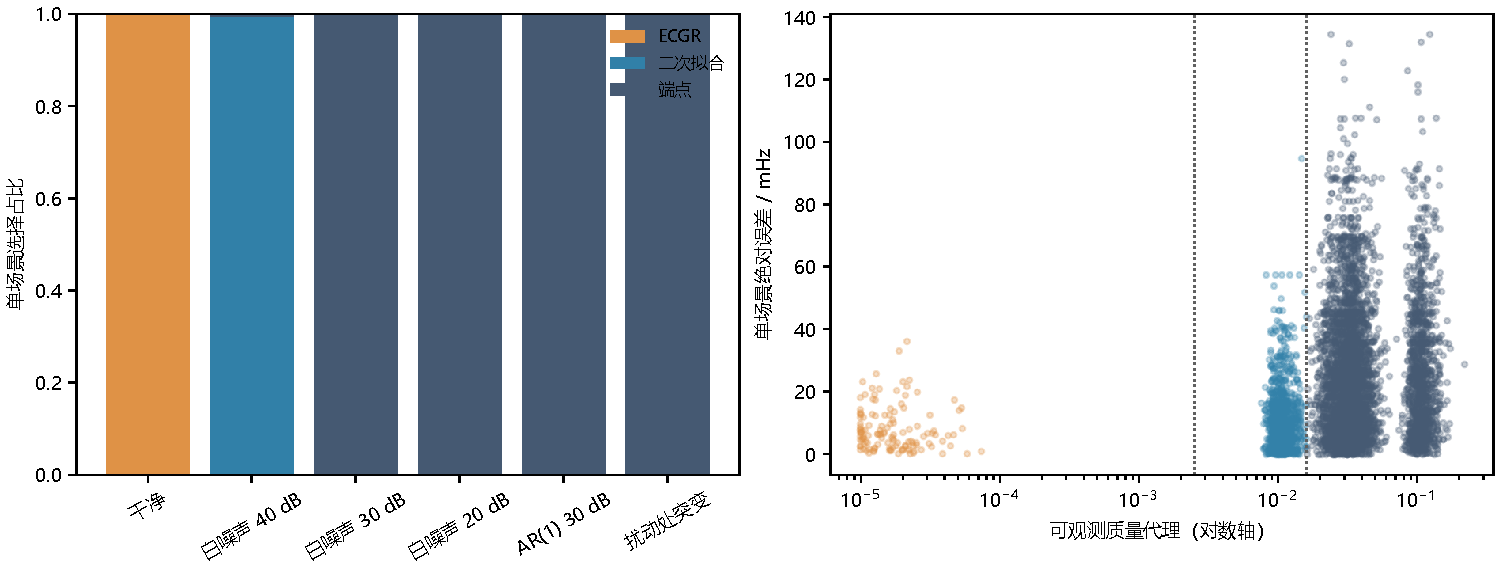
\includegraphics[width=.84\linewidth]{quality-assets/figures/quality-selection-performance.pdf}\captionof{figure}{固定截止独立确认。左为128个单场景在各条件的表示比例，右为质量代理与绝对误差；含噪条件每物理事件10个复本。}\label{fig:fixed-q}\end{center}

\begin{center}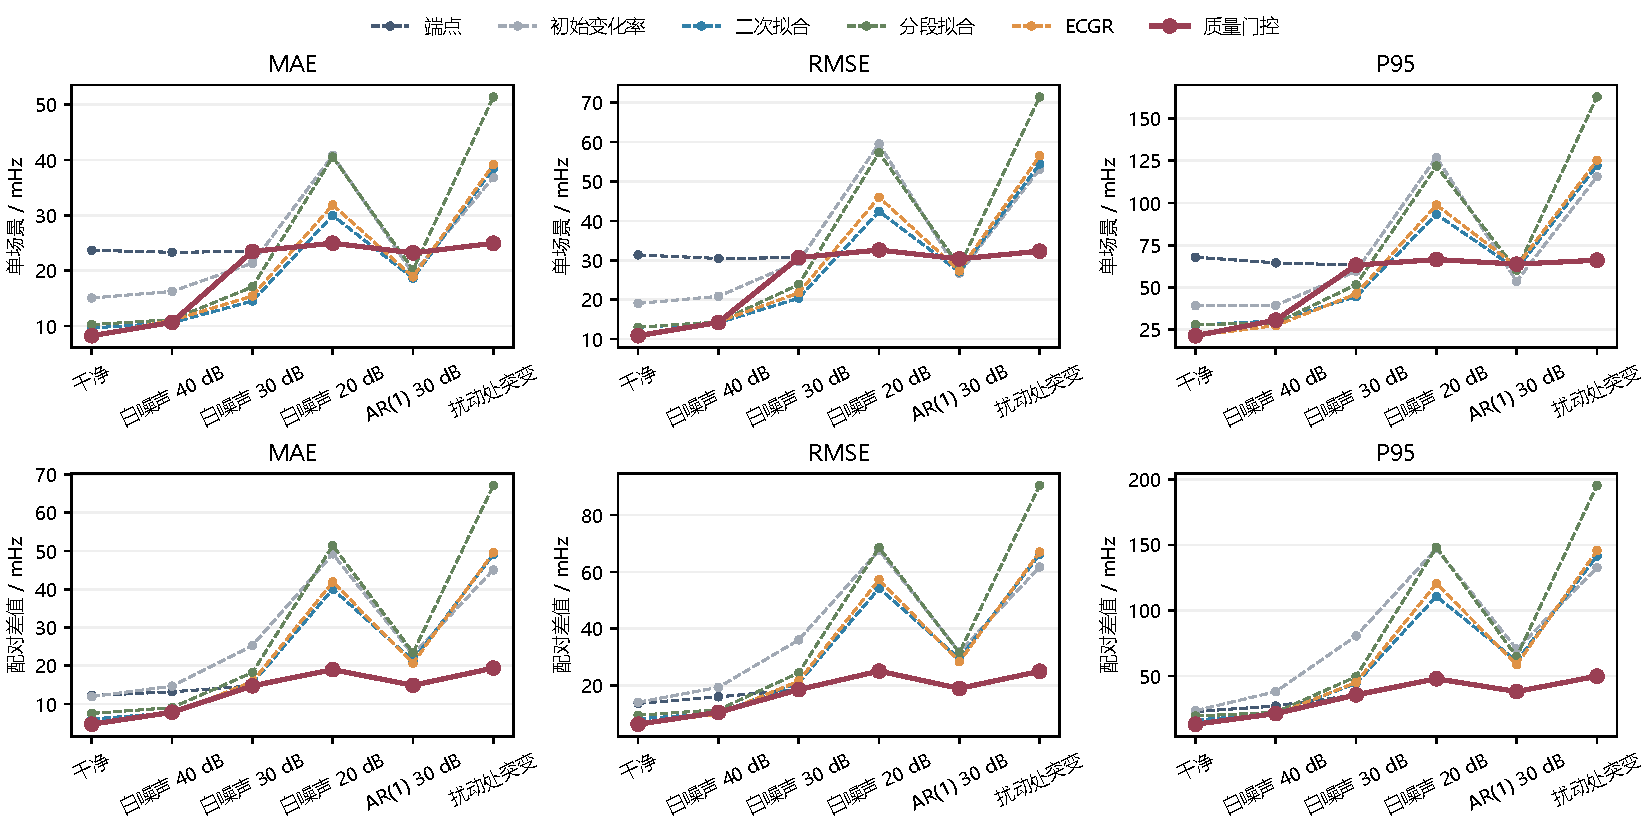
\includegraphics[width=.84\linewidth]{quality-assets/figures/quality-strategy-errors.pdf}\captionof{figure}{固定截止独立确认。上行为128个单场景，下行为220个主幅值配对，含噪条件每物理事件10个复本。误差单位为mHz。}\label{fig:fixed-errors}\end{center}

\clearpage\section{原滚动与固定时刻的逐事件分解}

\begin{table}[!htbp]\centering\small\setlength{\tabcolsep}{4pt}
\caption{原滚动与固定策略的集合分解。提前量只对各行中及时命中者统计，未越限组的分母为1309。}\label{tab:original-sets}
\begin{tabular}{lrrrrrrr}
\toprule
集合 & 物理事件 & 滚动命中 & 固定命中 & 滚动提前/ms & 固定提前/ms & 滚动虚警 & 固定虚警 \\
\midrule
全体越限 & 291 & 272 & 189 & 390 & 240 & 0 & 0 \\
首次越限 $\leq 0.50$ s & 98 & 98 & 0 & 240 & -- & 0 & 0 \\
首次越限 $>0.50$ s & 193 & 174 & 189 & 460 & 240 & 0 & 0 \\
共同命中 & 174 & 174 & 174 & 460 & 210 & 0 & 0 \\
仅滚动命中 & 98 & 98 & 0 & 240 & -- & 0 & 0 \\
仅固定命中 & 15 & 0 & 15 & -- & 560 & 0 & 0 \\
均未命中 & 4 & 0 & 0 & -- & -- & 0 & 0 \\
全部未越限 & 1309 & 0 & 0 & -- & -- & 84 & 74 \\
共同虚警 & 51 & 0 & 0 & -- & -- & 51 & 51 \\
仅滚动虚警 & 33 & 0 & 0 & -- & -- & 33 & 0 \\
仅固定虚警 & 23 & 0 & 0 & -- & -- & 0 & 23 \\
均未虚警 & 1202 & 0 & 0 & -- & -- & 0 & 0 \\
\bottomrule\end{tabular}\end{table}

固定0.50 s策略在193个晚越限事件中命中189个。早越限组没有固定策略可计算的及时提前量。虚警计算限于未越限事件，风险组逐集合不另造虚警分母。

\clearpage\section{滚动ECGR接入试验的完整工作点}

绝对值来自2400个物理事件。五种主量测等权，每个事件在各主条件各出现一次；混合分母为2045个越限和9955个未越限组合，突变单列。各单条件共有409个越限、1991个未越限。提前量只对本策略命中集合取中位数。标记“主”是预设10\%两策略，“次”是锁定5\%工作点，“分”是同规则分别分级校准的次要诊断，“事”是事后补表。持续性不是预设主要对照。

\begingroup\scriptsize\setlength{\tabcolsep}{3pt}
\begin{longtable}{lrlclrrrrr}
\caption{滚动接入各策略绝对工作点，比例为\%。分级阈值写作高质量/低质量。}\label{tab:transfer-full}\\
\toprule
量测 & 目标 & 策略 & 属性 & 阈值/Hz & 命中/越限 & 虚警/未越限 & 命中率 & 虚警率 & 提前/ms \\
\midrule\endfirsthead
\toprule
量测 & 目标 & 策略 & 属性 & 阈值/Hz & 命中/越限 & 虚警/未越限 & 命中率 & 虚警率 & 提前/ms \\
\midrule\endhead
\bottomrule\endfoot
主条件混合 & 10 & 门控滚动 & 主 & 49.7357 & 1622/2045 & 1076/9955 & 79.32 & 10.81 & 260 \\
主条件混合 & 10 & 二次滚动 & 主 & 49.6509 & 1012/2045 & 912/9955 & 49.49 & 9.16 & 320 \\
主条件混合 & 10 & 持续性滚动 & 事 & 49.8231 & 1673/2045 & 1036/9955 & 81.81 & 10.41 & 180 \\
主条件混合 & 10 & 端点滚动 & 事 & 49.7279 & 1288/2045 & 1005/9955 & 62.98 & 10.10 & 180 \\
主条件混合 & 10 & 固定ECGR & 事 & 49.6466 & 1219/2045 & 1012/9955 & 59.61 & 10.17 & 320 \\
主条件混合 & 10 & 仅末窗门控 & 事 & 49.6509 & 991/2045 & 910/9955 & 48.46 & 9.14 & 340 \\
主条件混合 & 10 & 分段滚动 & 事 & 49.6568 & 1042/2045 & 1012/9955 & 50.95 & 10.17 & 260 \\
主条件混合 & 10 & 0.50 s二次 & 事 & 49.7594 & 1390/2045 & 892/9955 & 67.97 & 8.96 & 220 \\
主条件混合 & 10 & 二次滚动（分级） & 分 & 49.7210/49.6008 & 1255/2045 & 900/9955 & 61.37 & 9.04 & 340 \\
主条件混合 & 10 & 门控滚动（分级） & 分 & 49.7475/49.7162 & 1435/2045 & 937/9955 & 70.17 & 9.41 & 300 \\
主条件混合 & 5 & 门控滚动 & 次 & 49.7177 & 1276/2045 & 385/9955 & 62.40 & 3.87 & 220 \\
主条件混合 & 5 & 二次滚动 & 次 & 49.6303 & 778/2045 & 541/9955 & 38.04 & 5.43 & 320 \\
主条件混合 & 5 & 持续性滚动 & 事 & 49.8058 & 1389/2045 & 556/9955 & 67.92 & 5.59 & 140 \\
主条件混合 & 5 & 端点滚动 & 事 & 49.7177 & 1105/2045 & 523/9955 & 54.03 & 5.25 & 160 \\
主条件混合 & 5 & 固定ECGR & 事 & 49.6185 & 902/2045 & 480/9955 & 44.11 & 4.82 & 280 \\
主条件混合 & 5 & 仅末窗门控 & 事 & 49.6303 & 763/2045 & 540/9955 & 37.31 & 5.42 & 320 \\
主条件混合 & 5 & 分段滚动 & 事 & 49.5953 & 574/2045 & 524/9955 & 28.07 & 5.26 & 260 \\
主条件混合 & 5 & 0.50 s二次 & 事 & 49.7401 & 1174/2045 & 432/9955 & 57.41 & 4.34 & 220 \\
主条件混合 & 5 & 二次滚动（分级） & 分 & 49.6509/49.5557 & 670/2045 & 456/9955 & 32.76 & 4.58 & 280 \\
主条件混合 & 5 & 门控滚动（分级） & 分 & 49.7271/49.7067 & 1151/2045 & 475/9955 & 56.28 & 4.77 & 240 \\
干净 & 10 & 门控滚动 & 主 & 49.7357 & 385/409 & 54/1991 & 94.13 & 2.71 & 400 \\
干净 & 10 & 二次滚动 & 主 & 49.6509 & 75/409 & 0/1991 & 18.34 & 0.00 & 200 \\
干净 & 10 & 持续性滚动 & 事 & 49.8231 & 336/409 & 198/1991 & 82.15 & 9.94 & 180 \\
干净 & 10 & 端点滚动 & 事 & 49.7279 & 257/409 & 207/1991 & 62.84 & 10.40 & 160 \\
干净 & 10 & 固定ECGR & 事 & 49.6466 & 67/409 & 0/1991 & 16.38 & 0.00 & 200 \\
干净 & 10 & 仅末窗门控 & 事 & 49.6509 & 75/409 & 0/1991 & 18.34 & 0.00 & 200 \\
干净 & 10 & 分段滚动 & 事 & 49.6568 & 86/409 & 0/1991 & 21.03 & 0.00 & 160 \\
干净 & 10 & 0.50 s二次 & 事 & 49.7594 & 300/409 & 125/1991 & 73.35 & 6.28 & 230 \\
干净 & 10 & 二次滚动（分级） & 分 & 49.7210/49.6008 & 307/409 & 8/1991 & 75.06 & 0.40 & 320 \\
干净 & 10 & 门控滚动（分级） & 分 & 49.7475/49.7162 & 404/409 & 108/1991 & 98.78 & 5.42 & 420 \\
干净 & 5 & 门控滚动 & 次 & 49.7177 & 301/409 & 7/1991 & 73.59 & 0.35 & 320 \\
干净 & 5 & 二次滚动 & 次 & 49.6303 & 50/409 & 0/1991 & 12.22 & 0.00 & 190 \\
干净 & 5 & 持续性滚动 & 事 & 49.8058 & 277/409 & 107/1991 & 67.73 & 5.37 & 140 \\
干净 & 5 & 端点滚动 & 事 & 49.7177 & 218/409 & 113/1991 & 53.30 & 5.68 & 130 \\
干净 & 5 & 固定ECGR & 事 & 49.6185 & 29/409 & 0/1991 & 7.09 & 0.00 & 200 \\
干净 & 5 & 仅末窗门控 & 事 & 49.6303 & 50/409 & 0/1991 & 12.22 & 0.00 & 190 \\
干净 & 5 & 分段滚动 & 事 & 49.5953 & 16/409 & 0/1991 & 3.91 & 0.00 & 120 \\
干净 & 5 & 0.50 s二次 & 事 & 49.7401 & 260/409 & 23/1991 & 63.57 & 1.16 & 220 \\
干净 & 5 & 二次滚动（分级） & 分 & 49.6509/49.5557 & 75/409 & 0/1991 & 18.34 & 0.00 & 200 \\
干净 & 5 & 门控滚动（分级） & 分 & 49.7271/49.7067 & 353/409 & 24/1991 & 86.31 & 1.21 & 360 \\
白40 dB & 10 & 门控滚动 & 主 & 49.7357 & 381/409 & 205/1991 & 93.15 & 10.30 & 280 \\
白40 dB & 10 & 二次滚动 & 主 & 49.6509 & 169/409 & 72/1991 & 41.32 & 3.62 & 280 \\
白40 dB & 10 & 持续性滚动 & 事 & 49.8231 & 336/409 & 200/1991 & 82.15 & 10.05 & 180 \\
白40 dB & 10 & 端点滚动 & 事 & 49.7279 & 253/409 & 205/1991 & 61.86 & 10.30 & 160 \\
白40 dB & 10 & 固定ECGR & 事 & 49.6466 & 252/409 & 116/1991 & 61.61 & 5.83 & 320 \\
白40 dB & 10 & 仅末窗门控 & 事 & 49.6509 & 169/409 & 72/1991 & 41.32 & 3.62 & 280 \\
白40 dB & 10 & 分段滚动 & 事 & 49.6568 & 129/409 & 22/1991 & 31.54 & 1.10 & 200 \\
白40 dB & 10 & 0.50 s二次 & 事 & 49.7594 & 300/409 & 134/1991 & 73.35 & 6.73 & 230 \\
白40 dB & 10 & 二次滚动（分级） & 分 & 49.7210/49.6008 & 348/409 & 176/1991 & 85.09 & 8.84 & 340 \\
白40 dB & 10 & 门控滚动（分级） & 分 & 49.7475/49.7162 & 402/409 & 289/1991 & 98.29 & 14.52 & 320 \\
白40 dB & 5 & 门控滚动 & 次 & 49.7177 & 302/409 & 70/1991 & 73.84 & 3.52 & 240 \\
白40 dB & 5 & 二次滚动 & 次 & 49.6303 & 107/409 & 35/1991 & 26.16 & 1.76 & 260 \\
白40 dB & 5 & 持续性滚动 & 事 & 49.8058 & 275/409 & 108/1991 & 67.24 & 5.42 & 140 \\
白40 dB & 5 & 端点滚动 & 事 & 49.7177 & 214/409 & 102/1991 & 52.32 & 5.12 & 140 \\
白40 dB & 5 & 固定ECGR & 事 & 49.6185 & 165/409 & 32/1991 & 40.34 & 1.61 & 240 \\
白40 dB & 5 & 仅末窗门控 & 事 & 49.6303 & 107/409 & 35/1991 & 26.16 & 1.76 & 260 \\
白40 dB & 5 & 分段滚动 & 事 & 49.5953 & 38/409 & 2/1991 & 9.29 & 0.10 & 210 \\
白40 dB & 5 & 0.50 s二次 & 事 & 49.7401 & 257/409 & 31/1991 & 62.84 & 1.56 & 220 \\
白40 dB & 5 & 二次滚动（分级） & 分 & 49.6509/49.5557 & 169/409 & 72/1991 & 41.32 & 3.62 & 280 \\
白40 dB & 5 & 门控滚动（分级） & 分 & 49.7271/49.7067 & 346/409 & 155/1991 & 84.60 & 7.79 & 260 \\
白30 dB & 10 & 门控滚动 & 主 & 49.7357 & 285/409 & 283/1991 & 69.68 & 14.21 & 220 \\
白30 dB & 10 & 二次滚动 & 主 & 49.6509 & 240/409 & 216/1991 & 58.68 & 10.85 & 340 \\
白30 dB & 10 & 持续性滚动 & 事 & 49.8231 & 334/409 & 212/1991 & 81.66 & 10.65 & 180 \\
白30 dB & 10 & 端点滚动 & 事 & 49.7279 & 261/409 & 212/1991 & 63.81 & 10.65 & 180 \\
白30 dB & 10 & 固定ECGR & 事 & 49.6466 & 298/409 & 261/1991 & 72.86 & 13.11 & 340 \\
白30 dB & 10 & 仅末窗门控 & 事 & 49.6509 & 235/409 & 216/1991 & 57.46 & 10.85 & 340 \\
白30 dB & 10 & 分段滚动 & 事 & 49.6568 & 246/409 & 173/1991 & 60.15 & 8.69 & 260 \\
白30 dB & 10 & 0.50 s二次 & 事 & 49.7594 & 284/409 & 166/1991 & 69.44 & 8.34 & 220 \\
白30 dB & 10 & 二次滚动（分级） & 分 & 49.7210/49.6008 & 176/409 & 258/1991 & 43.03 & 12.96 & 370 \\
白30 dB & 10 & 门控滚动（分级） & 分 & 49.7475/49.7162 & 198/409 & 226/1991 & 48.41 & 11.35 & 200 \\
白30 dB & 5 & 门控滚动 & 次 & 49.7177 & 217/409 & 114/1991 & 53.06 & 5.73 & 160 \\
白30 dB & 5 & 二次滚动 & 次 & 49.6303 & 191/409 & 132/1991 & 46.70 & 6.63 & 320 \\
白30 dB & 5 & 持续性滚动 & 事 & 49.8058 & 278/409 & 109/1991 & 67.97 & 5.47 & 140 \\
白30 dB & 5 & 端点滚动 & 事 & 49.7177 & 217/409 & 114/1991 & 53.06 & 5.73 & 160 \\
白30 dB & 5 & 固定ECGR & 事 & 49.6185 & 220/409 & 118/1991 & 53.79 & 5.93 & 280 \\
白30 dB & 5 & 仅末窗门控 & 事 & 49.6303 & 189/409 & 132/1991 & 46.21 & 6.63 & 340 \\
白30 dB & 5 & 分段滚动 & 事 & 49.5953 & 131/409 & 54/1991 & 32.03 & 2.71 & 260 \\
白30 dB & 5 & 0.50 s二次 & 事 & 49.7401 & 238/409 & 62/1991 & 58.19 & 3.11 & 220 \\
白30 dB & 5 & 二次滚动（分级） & 分 & 49.6509/49.5557 & 109/409 & 120/1991 & 26.65 & 6.03 & 340 \\
白30 dB & 5 & 门控滚动（分级） & 分 & 49.7271/49.7067 & 142/409 & 134/1991 & 34.72 & 6.73 & 160 \\
白20 dB & 10 & 门控滚动 & 主 & 49.7357 & 289/409 & 283/1991 & 70.66 & 14.21 & 240 \\
白20 dB & 10 & 二次滚动 & 主 & 49.6509 & 290/409 & 403/1991 & 70.90 & 20.24 & 340 \\
白20 dB & 10 & 持续性滚动 & 事 & 49.8231 & 330/409 & 219/1991 & 80.68 & 11.00 & 200 \\
白20 dB & 10 & 端点滚动 & 事 & 49.7279 & 260/409 & 207/1991 & 63.57 & 10.40 & 220 \\
白20 dB & 10 & 固定ECGR & 事 & 49.6466 & 325/409 & 452/1991 & 79.46 & 22.70 & 340 \\
白20 dB & 10 & 仅末窗门控 & 事 & 49.6509 & 280/409 & 401/1991 & 68.46 & 20.14 & 360 \\
白20 dB & 10 & 分段滚动 & 事 & 49.6568 & 351/409 & 717/1991 & 85.82 & 36.01 & 340 \\
白20 dB & 10 & 0.50 s二次 & 事 & 49.7594 & 234/409 & 269/1991 & 57.21 & 13.51 & 200 \\
白20 dB & 10 & 二次滚动（分级） & 分 & 49.7210/49.6008 & 214/409 & 146/1991 & 52.32 & 7.33 & 320 \\
白20 dB & 10 & 门控滚动（分级） & 分 & 49.7475/49.7162 & 212/409 & 90/1991 & 51.83 & 4.52 & 220 \\
白20 dB & 5 & 门控滚动 & 次 & 49.7177 & 233/409 & 103/1991 & 56.97 & 5.17 & 200 \\
白20 dB & 5 & 二次滚动 & 次 & 49.6303 & 252/409 & 253/1991 & 61.61 & 12.71 & 340 \\
白20 dB & 5 & 持续性滚动 & 事 & 49.8058 & 276/409 & 122/1991 & 67.48 & 6.13 & 140 \\
白20 dB & 5 & 端点滚动 & 事 & 49.7177 & 233/409 & 103/1991 & 56.97 & 5.17 & 200 \\
白20 dB & 5 & 固定ECGR & 事 & 49.6185 & 278/409 & 243/1991 & 67.97 & 12.20 & 320 \\
白20 dB & 5 & 仅末窗门控 & 事 & 49.6303 & 242/409 & 252/1991 & 59.17 & 12.66 & 340 \\
白20 dB & 5 & 分段滚动 & 事 & 49.5953 & 290/409 & 442/1991 & 70.90 & 22.20 & 320 \\
白20 dB & 5 & 0.50 s二次 & 事 & 49.7401 & 190/409 & 208/1991 & 46.45 & 10.45 & 200 \\
白20 dB & 5 & 二次滚动（分级） & 分 & 49.6509/49.5557 & 172/409 & 107/1991 & 42.05 & 5.37 & 280 \\
白20 dB & 5 & 门控滚动（分级） & 分 & 49.7271/49.7067 & 158/409 & 51/1991 & 38.63 & 2.56 & 160 \\
AR(1)30 dB & 10 & 门控滚动 & 主 & 49.7357 & 282/409 & 251/1991 & 68.95 & 12.61 & 200 \\
AR(1)30 dB & 10 & 二次滚动 & 主 & 49.6509 & 238/409 & 221/1991 & 58.19 & 11.10 & 380 \\
AR(1)30 dB & 10 & 持续性滚动 & 事 & 49.8231 & 337/409 & 207/1991 & 82.40 & 10.40 & 180 \\
AR(1)30 dB & 10 & 端点滚动 & 事 & 49.7279 & 257/409 & 174/1991 & 62.84 & 8.74 & 160 \\
AR(1)30 dB & 10 & 固定ECGR & 事 & 49.6466 & 277/409 & 183/1991 & 67.73 & 9.19 & 320 \\
AR(1)30 dB & 10 & 仅末窗门控 & 事 & 49.6509 & 232/409 & 221/1991 & 56.72 & 11.10 & 380 \\
AR(1)30 dB & 10 & 分段滚动 & 事 & 49.6568 & 230/409 & 100/1991 & 56.23 & 5.02 & 280 \\
AR(1)30 dB & 10 & 0.50 s二次 & 事 & 49.7594 & 272/409 & 198/1991 & 66.50 & 9.94 & 220 \\
AR(1)30 dB & 10 & 二次滚动（分级） & 分 & 49.7210/49.6008 & 210/409 & 312/1991 & 51.34 & 15.67 & 420 \\
AR(1)30 dB & 10 & 门控滚动（分级） & 分 & 49.7475/49.7162 & 219/409 & 224/1991 & 53.55 & 11.25 & 220 \\
AR(1)30 dB & 5 & 门控滚动 & 次 & 49.7177 & 223/409 & 91/1991 & 54.52 & 4.57 & 140 \\
AR(1)30 dB & 5 & 二次滚动 & 次 & 49.6303 & 178/409 & 121/1991 & 43.52 & 6.08 & 350 \\
AR(1)30 dB & 5 & 持续性滚动 & 事 & 49.8058 & 283/409 & 110/1991 & 69.19 & 5.52 & 140 \\
AR(1)30 dB & 5 & 端点滚动 & 事 & 49.7177 & 223/409 & 91/1991 & 54.52 & 4.57 & 140 \\
AR(1)30 dB & 5 & 固定ECGR & 事 & 49.6185 & 210/409 & 87/1991 & 51.34 & 4.37 & 280 \\
AR(1)30 dB & 5 & 仅末窗门控 & 事 & 49.6303 & 175/409 & 121/1991 & 42.79 & 6.08 & 360 \\
AR(1)30 dB & 5 & 分段滚动 & 事 & 49.5953 & 99/409 & 26/1991 & 24.21 & 1.31 & 240 \\
AR(1)30 dB & 5 & 0.50 s二次 & 事 & 49.7401 & 229/409 & 108/1991 & 55.99 & 5.42 & 220 \\
AR(1)30 dB & 5 & 二次滚动（分级） & 分 & 49.6509/49.5557 & 145/409 & 157/1991 & 35.45 & 7.89 & 360 \\
AR(1)30 dB & 5 & 门控滚动（分级） & 分 & 49.7271/49.7067 & 152/409 & 111/1991 & 37.16 & 5.58 & 180 \\
噪声突变 & 10 & 门控滚动 & 主 & 49.7357 & 288/409 & 252/1991 & 70.42 & 12.66 & 240 \\
噪声突变 & 10 & 二次滚动 & 主 & 49.6509 & 291/409 & 389/1991 & 71.15 & 19.54 & 360 \\
噪声突变 & 10 & 持续性滚动 & 事 & 49.8231 & 331/409 & 211/1991 & 80.93 & 10.60 & 180 \\
噪声突变 & 10 & 端点滚动 & 事 & 49.7279 & 263/409 & 196/1991 & 64.30 & 9.84 & 200 \\
噪声突变 & 10 & 固定ECGR & 事 & 49.6466 & 318/409 & 349/1991 & 77.75 & 17.53 & 340 \\
噪声突变 & 10 & 仅末窗门控 & 事 & 49.6509 & 272/409 & 379/1991 & 66.50 & 19.04 & 380 \\
噪声突变 & 10 & 分段滚动 & 事 & 49.6568 & 343/409 & 586/1991 & 83.86 & 29.43 & 340 \\
噪声突变 & 10 & 0.50 s二次 & 事 & 49.7594 & 221/409 & 325/1991 & 54.03 & 16.32 & 200 \\
噪声突变 & 10 & 二次滚动（分级） & 分 & 49.7210/49.6008 & 338/409 & 617/1991 & 82.64 & 30.99 & 380 \\
噪声突变 & 10 & 门控滚动（分级） & 分 & 49.7475/49.7162 & 316/409 & 334/1991 & 77.26 & 16.78 & 280 \\
噪声突变 & 5 & 门控滚动 & 次 & 49.7177 & 241/409 & 105/1991 & 58.92 & 5.27 & 180 \\
噪声突变 & 5 & 二次滚动 & 次 & 49.6303 & 255/409 & 236/1991 & 62.35 & 11.85 & 340 \\
噪声突变 & 5 & 持续性滚动 & 事 & 49.8058 & 277/409 & 115/1991 & 67.73 & 5.78 & 140 \\
噪声突变 & 5 & 端点滚动 & 事 & 49.7177 & 241/409 & 104/1991 & 58.92 & 5.22 & 180 \\
噪声突变 & 5 & 固定ECGR & 事 & 49.6185 & 269/409 & 207/1991 & 65.77 & 10.40 & 320 \\
噪声突变 & 5 & 仅末窗门控 & 事 & 49.6303 & 235/409 & 226/1991 & 57.46 & 11.35 & 340 \\
噪声突变 & 5 & 分段滚动 & 事 & 49.5953 & 270/409 & 317/1991 & 66.01 & 15.92 & 330 \\
噪声突变 & 5 & 0.50 s二次 & 事 & 49.7401 & 187/409 & 262/1991 & 45.72 & 13.16 & 220 \\
噪声突变 & 5 & 二次滚动（分级） & 分 & 49.6509/49.5557 & 291/409 & 389/1991 & 71.15 & 19.54 & 360 \\
噪声突变 & 5 & 门控滚动（分级） & 分 & 49.7271/49.7067 & 263/409 & 194/1991 & 64.30 & 9.74 & 200 \\
\end{longtable}\endgroup

\begingroup\scriptsize\setlength{\tabcolsep}{3pt}
\begin{longtable}{rlrrr}
\caption{冻结告警阈值（Hz）。分级策略读同一可观测质量标记，并各自使用高低质量阈值；其全局阈值只作回退。}\label{tab:transfer-cutoffs}\\
\toprule
目标/\% & 策略 & 全局阈值 & 高质量阈值 & 低质量阈值 \\
\midrule\endfirsthead
\toprule
目标/\% & 策略 & 全局阈值 & 高质量阈值 & 低质量阈值 \\
\midrule\endhead
\bottomrule\endfoot
10 & 门控滚动 & 49.735736704 & -- & -- \\
10 & 二次滚动 & 49.650896263 & -- & -- \\
10 & 持续性滚动 & 49.823098068 & -- & -- \\
10 & 端点滚动 & 49.727883230 & -- & -- \\
10 & 固定ECGR & 49.646637037 & -- & -- \\
10 & 仅末窗门控 & 49.650896263 & -- & -- \\
10 & 分段滚动 & 49.656803125 & -- & -- \\
10 & 0.50 s二次 & 49.759387190 & -- & -- \\
10 & 二次滚动（分级） & 49.650896263 & 49.721007404 & 49.600753317 \\
10 & 门控滚动（分级） & 49.735736704 & 49.747514752 & 49.716156673 \\
5 & 门控滚动 & 49.717730793 & -- & -- \\
5 & 二次滚动 & 49.630338868 & -- & -- \\
5 & 持续性滚动 & 49.805799076 & -- & -- \\
5 & 端点滚动 & 49.717730793 & -- & -- \\
5 & 固定ECGR & 49.618502976 & -- & -- \\
5 & 仅末窗门控 & 49.630338868 & -- & -- \\
5 & 分段滚动 & 49.595318684 & -- & -- \\
5 & 0.50 s二次 & 49.740126325 & -- & -- \\
5 & 二次滚动（分级） & 49.630338868 & 49.650896263 & 49.555714640 \\
5 & 门控滚动（分级） & 49.717730793 & 49.727068374 & 49.706721537 \\
\end{longtable}\endgroup

\clearpage

\begin{table}[!htbp]\centering\small\setlength{\tabcolsep}{4pt}
\caption{10\%校准目标的预设比较。正差为门控指标更高，虚警正差表示代价。事件簇为2400个物理事件，区间为95\%。}\label{tab:transfer-effects}
\begin{tabular}{lrr}
\toprule
条件 & 命中差/百分点 & 虚警差/百分点 \\
\midrule
主条件混合 & 29.83 [26.46, 33.10] & 1.65 [0.72, 2.58] \\
干净 & 75.79 [71.63, 79.86] & 2.71 [2.01, 3.48] \\
白40 dB & 51.83 [46.98, 56.96] & 6.68 [5.27, 8.17] \\
白30 dB & 11.00 [4.71, 17.05] & 3.37 [1.56, 5.11] \\
白20 dB & −0.24 [−5.77, 5.50] & −6.03 [−8.01, −4.06] \\
AR(1)30 dB & 10.76 [4.73, 16.90] & 1.51 [−0.20, 3.30] \\
噪声突变 & −0.73 [−6.67, 4.99] & −6.88 [−8.78, −4.97] \\
\bottomrule\end{tabular}\end{table}

两种比例的区间按4000次物理事件配对重采样。混合虚警差区间上限2.58个百分点超过预设2个百分点，主验收未通过（三项通过、一项失败）。10\%目标下，门控相对同批持续性的命中差为−2.49、虚警差为0.40个百分点，配对区间分别为[−5.41, 0.38]、[−0.57, 1.34]。其余策略与两档工作点的配对区间见随附联合结果表。

\begin{center}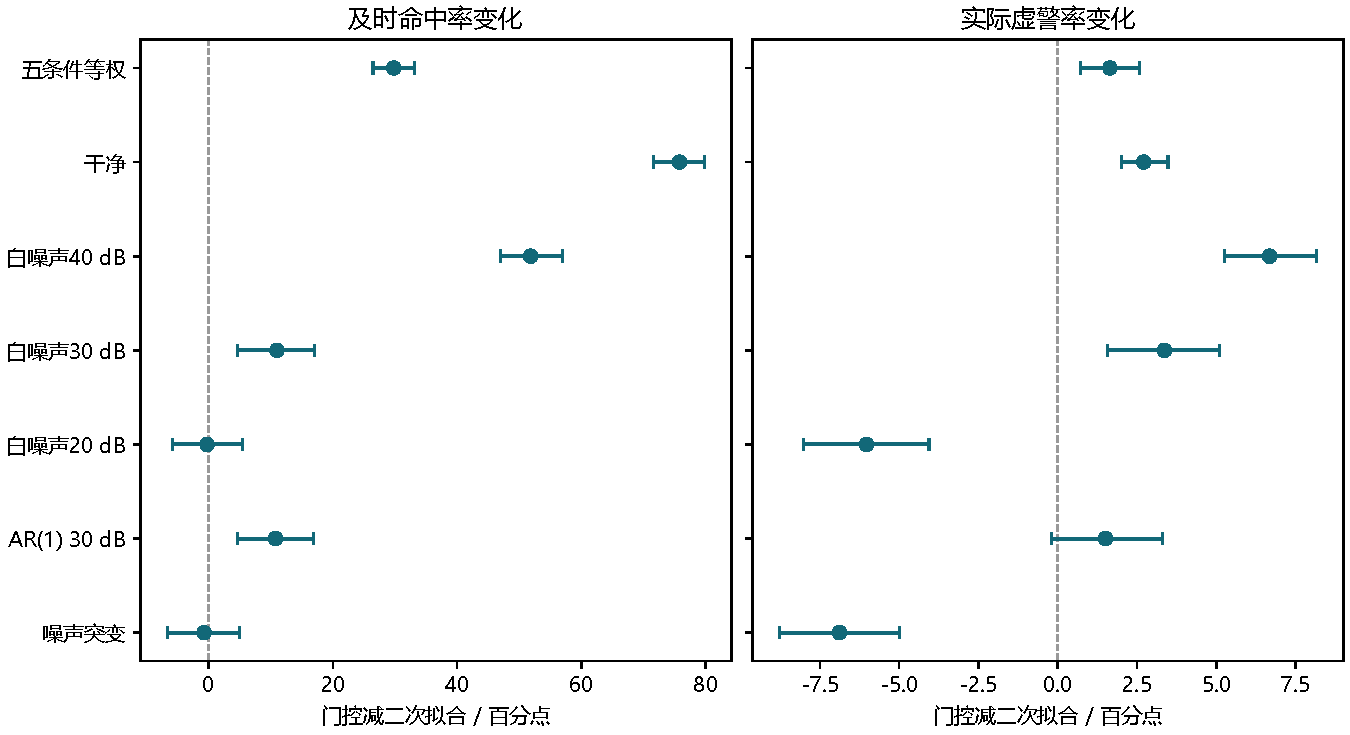
\includegraphics[width=.84\linewidth]{rolling-figures/paired-event-effects.pdf}\captionof{figure}{10\%校准目标下预设主要比较的量测分层效应。门控减二次滚动，横坐标为百分点；线段为以2400个物理事件为簇的95\%区间。}\label{fig:transfer-effect}\end{center}

\clearpage

\begin{center}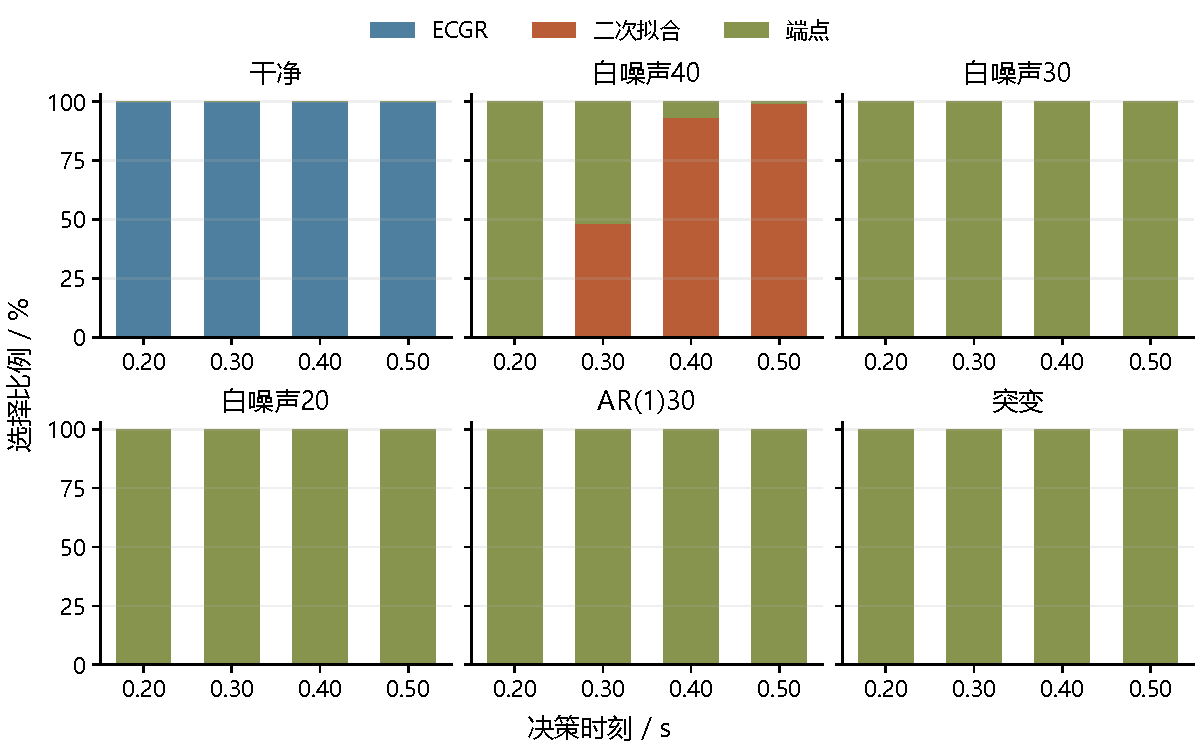
\includegraphics[width=.87\linewidth]{audit-figures/rolling-discrete-selection.pdf}\captionof{figure}{2400个物理事件在四个决策窗的离散选择比例，每柱分母为2400。分层来自模拟量测标签，选择只用当前窗与共用扰动前量测。}\label{fig:transfer-select}\end{center}

\begin{center}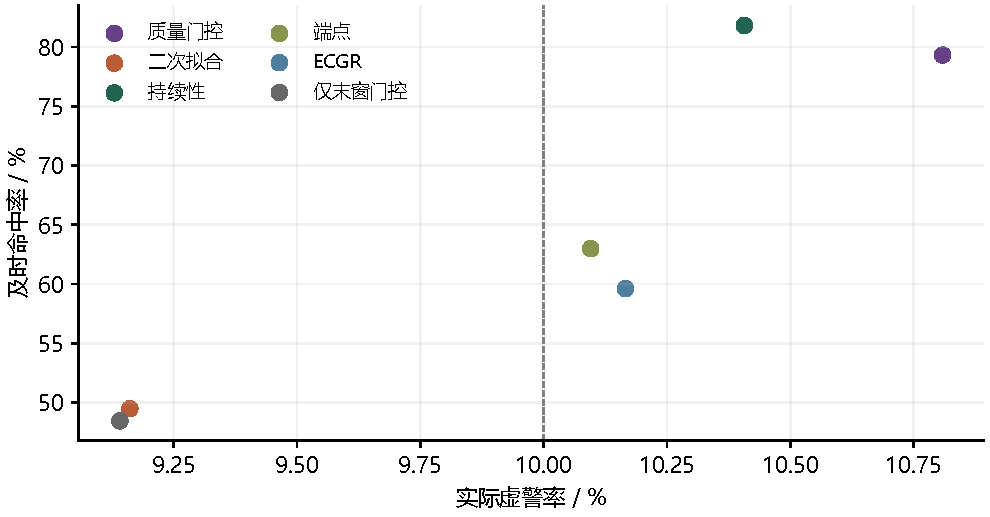
\includegraphics[width=.77\linewidth]{audit-figures/rolling-operating-points.pdf}\captionof{figure}{10\%校准目标下五种主条件等权的实测工作点。命中和虚警的分母分别为2045和9955个组合；持续性等为非主对照，绝对结果见表\ref{tab:transfer-full}。}\label{fig:transfer-op}\end{center}

\clearpage\section{告警工作点的事后诊断}

绝对阈值互换在原10\%全局阈值上做二乘二对照。用两种评分分别套用两个阈值，分别得到四个命中率；将阈值变化在两种评分上取平均，再将评分变化在两个阈值上取平均，两项之和等于原差。这个分解依赖使用同一绝对Hz刻度及原测试集，属于描述性诊断。

\begin{table}[!htbp]\centering\small\setlength{\tabcolsep}{4pt}
\caption{干净量测下同一评分使用两个固定阈值的诊断。分母为409个越限和1991个未越限。}\label{tab:threshold-swap}
\begin{tabular}{llrrrrr}
\toprule
评分 & 阈值来源 & 阈值/Hz & 命中 & 虚警 & 命中率/\% & 虚警率/\% \\
\midrule
二次滚动 & 二次滚动 & 49.650896 & 75 & 0 & 18.34 & 0.00 \\
二次滚动 & 门控滚动 & 49.735737 & 379 & 45 & 92.67 & 2.26 \\
门控滚动 & 二次滚动 & 49.650896 & 71 & 0 & 17.36 & 0.00 \\
门控滚动 & 门控滚动 & 49.735737 & 385 & 54 & 94.13 & 2.71 \\
\bottomrule\end{tabular}\end{table}

同实际虚警诊断预先只用5\%、10\%两个坐标。未越限事件用全部可用窗的最小值，越限事件用首次越限前各窗最小值；无可及时出分的越限事件仍留在分母。按预测值升序纳入同分组；虚警率平台取最早阈值，从不告警原点开始。在相邻可达虚警率之间线性插值，禁止外推，无法形成括点的复本标为不可用。区间由4000次配对物理事件重采样获得，每次重新构造插值括点，所有复本均可插值。诊断使用测试记录，不能用来重新校准主要阈值。

\begin{table}[!htbp]\centering\small\setlength{\tabcolsep}{4pt}
\caption{相同实际虚警率下的成对事后诊断。前两组为门控减二次滚动，原滚动组为滚动减固定时刻。}\label{tab:matched-far}
\begin{tabular}{lrrrrr}
\toprule
数据 & 实际虚警/\% & 策略命中/\% & 对照命中/\% & 命中差/百分点 & 95\%区间 \\
\midrule
新增混合 & 5 & 63.09 & 37.04 & 26.04 & [22.61, 29.57] \\
新增混合 & 10 & 77.79 & 49.93 & 27.86 & [22.84, 31.27] \\
新增干净 & 5 & 98.53 & 96.82 & 1.71 & [0.24, 3.75] \\
新增干净 & 10 & 99.52 & 99.51 & 0.01 & [−0.24, 0.72] \\
原滚动干净 & 5 & 91.41 & 63.92 & 27.49 & [20.64, 34.01] \\
原滚动干净 & 10 & 98.61 & 65.98 & 32.63 & [26.91, 38.38] \\
\bottomrule\end{tabular}\end{table}

\clearpage\section{同输入配对诊断与组件对照}
配对、训练和量测均复用固定截止ECGR确认的存档。完整窗树以26点频率为输入，物理模型对照选取使可见窗平方误差最小的训练参数组并读取其仿真后缀，同分取训练库行序在前者。用于配对估计的训练集为原692个场景。去白化将弦线残差权重改为单位阵，去三次项仅保留对称基，去收缩令三次项惩罚为零。三种配置各自按原数据划分和相同树容量重新拟合。去白化同时改变残差噪声尺度的估计，差值反映该整项操作。按下垂系数分带对96个参考事件聚类重采样5000次。消融是对已查看配对的事后分析。
\begin{center}\small\setlength{\tabcolsep}{4pt}
\captionof{table}{同输入的配对差值误差与方向判对。MAE、P95及差值区间以mHz计。最后一列是各配置减完整ECGR的MAE差的95\%区间。}\label{tab:abl-new}
\begin{tabular}{llrrrr}\toprule
量测 & 配置 & MAE & P95 & 方向正确/总数 & 差值区间 \\ \midrule
干净 & 完整ECGR & 4.44 & 11.20 & 234/288 & 参照 \\
干净 & 二次拟合 & 5.67 & 14.89 & 246/288 & $[0.75, 1.68]$ \\
干净 & 完整窗树 & 9.93 & 23.83 & 146/288 & $[4.63, 6.38]$ \\
干净 & 物理参数库 & 17.29 & 47.23 & 132/288 & $[10.79, 14.97]$ \\
干净 & 去白化 & 4.61 & 12.67 & 231/288 & $[-0.08, 0.41]$ \\
干净 & 去三次项 & 4.29 & 12.37 & 247/288 & $[-0.36, 0.05]$ \\
干净 & 去收缩 & 4.37 & 10.79 & 235/288 & $[-0.21, 0.07]$ \\
白噪30 dB & 完整ECGR & 13.96 & 39.57 & 1967/2880 & 参照 \\
白噪30 dB & 二次拟合 & 13.71 & 39.09 & 1944/2880 & $[-0.59, 0.08]$ \\
白噪30 dB & 完整窗树 & 13.94 & 38.00 & 1732/2880 & $[-0.84, 0.76]$ \\
白噪30 dB & 物理参数库 & 18.88 & 48.74 & 1369/2880 & $[3.03, 6.81]$ \\
白噪30 dB & 去白化 & 19.64 & 54.04 & 1820/2880 & $[5.11, 6.28]$ \\
白噪30 dB & 去三次项 & 14.00 & 39.92 & 1975/2880 & $[-0.09, 0.17]$ \\
白噪30 dB & 去收缩 & 16.11 & 43.25 & 1882/2880 & $[1.76, 2.53]$ \\
\bottomrule\end{tabular}\end{center}

\begin{center}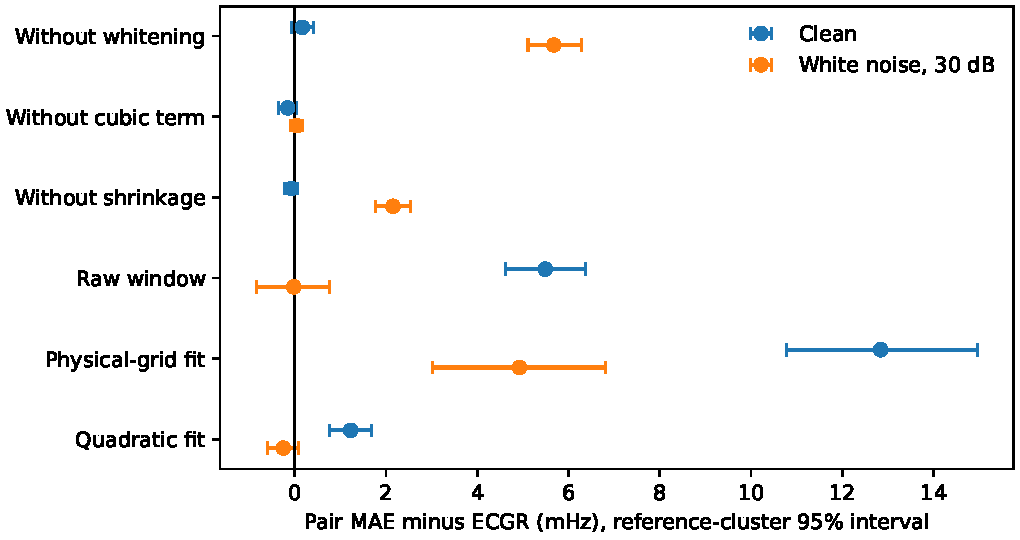
\includegraphics[width=.90\linewidth]{decision-assets/pair-ablation.pdf}
\captionof{figure}{同一批近端点配对上各配置相对完整ECGR的差值MAE变化，正值表示幅值误差增加。干净条件含222个主幅值配对，白噪声条件含其10个量测复本。横线为参考事件聚类95\%区间。}\label{fig:abl-new}\end{center}

\clearpage\section{最低提前量确认与跨系统压力结果}
开发在原滚动迁移的800个校准事件上完成，按预先指定的200 ms最低提前量比较64种映射，优先选有效命中较多者，同分时选择表示种数较少者，再按固定枚举次序。有效质量区间的分界为0.0025和0.016。质量无效时决策目标门控退回持续性，原幅值门控退回端点；本批有限质量代理下两者逐事件预测相同。用于滚动对照的完整窗树、去组件树和物理库沿用1200组聚合训练轨迹，输入仅含各自当前可见窗的11、16、21或26点。辅助树采用100棵深度3的提升树。门控还利用扰动前的50点量测形成质量代理。

新校准与确认块分别含800及2400个物理事件。各策略阈值分别在校准块上确定。主量测为干净、40/30/20 dB白噪声及30 dB等功率AR(1)，在每个物理事件内等权；从40 dB白噪声突变为20 dB相关噪声的变体单列。发报须满足评分严格低于策略阈值。提前量按毫秒计算，$\ell=200$ ms时恰好提前200 ms计为有效。无法及时出分的越限事件保留在分母。
\begin{center}\small\setlength{\tabcolsep}{4pt}
\captionof{table}{冻结校准阈值下至少提前200 ms的绝对计数。阈值为50 Hz等值尺度，提前量仅对各策略的有效命中取中位数。}\label{tab:abs-new}
\begin{tabular}{llrrrr}\toprule
数据 & 策略 & 阈值/Hz & 有效命中/越限 & 虚警/未越限 & 提前/ms \\ \midrule
聚合混合 & 质量门控 & 49.73574 & 1083/2005 & 994/9995 & 320 \\
聚合混合 & 持续性 & 49.82207 & 758/2005 & 1102/9995 & 260 \\
聚合混合 & 二次拟合 & 49.67653 & 964/2005 & 1099/9995 & 380 \\
聚合混合 & 完整ECGR & 49.65334 & 1105/2005 & 1100/9995 & 360 \\
聚合混合 & 完整窗树 & 49.73403 & 1140/2005 & 947/9995 & 320 \\
聚合混合 & 物理参数库 & 49.67898 & 651/2005 & 912/9995 & 340 \\
聚合突变 & 质量门控 & 49.73574 & 162/401 & 261/1999 & 300 \\
聚合突变 & 持续性 & 49.82207 & 156/401 & 221/1999 & 270 \\
聚合突变 & 二次拟合 & 49.67653 & 268/401 & 463/1999 & 400 \\
聚合突变 & 完整ECGR & 49.65334 & 291/401 & 405/1999 & 380 \\
聚合突变 & 完整窗树 & 49.73403 & 256/401 & 386/1999 & 360 \\
聚合突变 & 物理参数库 & 49.67898 & 181/401 & 281/1999 & 360 \\
多机回顾 & 质量门控 & 49.73574 & 0/350 & 0/240 & — \\
多机回顾 & 持续性 & 49.82207 & 0/350 & 0/240 & — \\
多机回顾 & 二次拟合 & 49.67653 & 0/350 & 0/240 & — \\
多机回顾 & 完整ECGR & 49.65334 & 0/350 & 0/240 & — \\
多机回顾 & 完整窗树 & 49.73403 & 0/350 & 0/240 & — \\
多机回顾 & 物理参数库 & 49.67898 & 0/350 & 0/240 & — \\
\bottomrule\end{tabular}\end{center}

\clearpage
新聚合确认要求，在冻结工作点相对持续性及开发期最佳简单参照的有效命中增量至少2个百分点、其95\%下限大于零，虚警增量的95\%上限不超过2个百分点，实测虚警率不超过12\%，并且等实际10\%虚警下的有效命中增量95\%下限大于零。开发选出的最佳简单参照也是持续性。在五种主量测的冻结阈值下，门控减持续性的有效命中率差为$+16.21$个百分点（95\%区间$[12.28,20.17]$），实际虚警率差为$-1.08$个百分点（$[-2.05,-0.09]$）。外部压力沿用聚合映射和阈值。其10个未收敛场景保留在设计账本，以下多机指标以完成求解的118个物理事件为条件。

\begin{center}\small\setlength{\tabcolsep}{4pt}
\captionof{table}{测试曲线等虚警诊断中门控减持续性的有效命中率差。各率按测试标签在10\%实际虚警率处插值，差及其区间以百分点计。0 ms仍要求严格早于越限。}\label{tab:roc-new}
\begin{tabular}{lrrrrr}\toprule
数据 & 时限/ms & 门控/\% & 持续性/\% & 差 & 95\%区间 \\ \midrule
原迁移档案 & 0 & 77.79 & 81.47 & -3.68 & $[-6.77, 0.94]$ \\
原迁移档案 & 100 & 68.20 & 73.42 & -5.22 & — \\
原迁移档案 & 200 & 50.89 & 39.22 & 11.68 & $[6.64, 20.12]$ \\
原迁移档案 & 300 & 33.97 & 13.59 & 20.38 & — \\
新聚合确认 & 0 & 79.27 & 79.43 & -0.16 & $[-4.11, 3.46]$ \\
新聚合确认 & 100 & 72.04 & 69.25 & 2.79 & — \\
新聚合确认 & 200 & 54.03 & 32.62 & 21.41 & $[14.19, 26.05]$ \\
新聚合确认 & 300 & 31.94 & 9.98 & 21.96 & — \\
多机高负荷 & 0 & 52.86 & 100.00 & -47.14 & $[-57.23, -37.22]$ \\
多机高负荷 & 100 & 52.86 & 100.00 & -47.14 & — \\
多机高负荷 & 200 & 52.86 & 100.00 & -47.14 & $[-57.23, -37.22]$ \\
多机高负荷 & 300 & 52.86 & 100.00 & -47.14 & — \\
\bottomrule\end{tabular}\end{center}

相同评分整组纳入，虚警计数平台取最先到达点。5\%及10\%坐标在相邻可达点间插值，不外推；每次物理事件簇重采样重新计算插值点。表中区间由2000次配对重采样得到，仅对0与200 ms计算。这里的插值命中率与上一表的冻结阈值整数计数有不同用途。前者刻画评分排序，后者同时反映校准阈值在测试工况中的适用性。


\clearpage\section{同一确认集上完整窗树与门控的事后对照}
以同一组2400个聚合物理事件的五种主量测为单位对齐两种策略的评分。末窗误差使用全部12000个变体；有效命中和虚警分别使用2005个越限变体和9995个未越限变体。首次告警须由严格低于各自冻结阈值的可见窗触发，有效命中须至少提前200 ms。每次有放回抽取2400个物理事件并保留簇内全部变体，分别重算三个比率的分子与分母。表中为5000次配对重采样的边际百分位区间。本项为既有确认集上的事后分析。

\begin{center}
\captionof{table}{完整窗树减质量门控的配对差异。末窗标签为0.50 s截止后最低频率，告警使用四窗首次触发。}\label{tab:raw-paired}
\begin{tabular}{lrrr}\toprule
指标 & 配对差 & 95\%下限 & 95\%上限 \\ \midrule
末窗MAE / mHz & 1.16 & 0.79 & 1.55 \\
有效命中率 / 百分点 & 2.84 & -0.30 & 5.87 \\
虚警率 / 百分点 & -0.47 & -1.16 & 0.18 \\
\bottomrule\end{tabular}\end{center}
完整窗树独有和门控独有的有效命中分别为405和348个，独有虚警分别为447和494个。沿用同一校准锁，直接在每个事件上比较完整窗树与门控可保留两种决策结果的相关性。原聚合确认以持续性作为主要简单对照，本表单独描述已查看数据上的表示比较。

\paragraph{历史表10的阈值读取精度} 校准集3355个未越限变体的逐事件最小门控评分按原阶次规则得到49.735736703583484 Hz。历史确认程序用 pandas 默认解析器重读阈值文件，实际比较值为49.73573670358349 Hz。用两个值分别严格比较同一批评分，校准端有330和339个虚警（9.84\%和10.10\%）。五种主量测确认端分别有1615和1622个及时命中、1036和1076个虚警。后者逐键复现12000条历史首报记录。表10沿用实际执行结果及其原验收；表S24的干净门控自阈值格在两种精度下均为385次命中、54次虚警。新确认由MAT文件加载阈值。
\end{document}